% start the document

% specify the document layout and font size
% \documentclass[preprint,12pt]{elsarticle}
\documentclass[final,twocolumn,12pt]{elsarticle}
\usepackage[margin=1.5cm,includefoot]{geometry}
\usepackage{setspace}

% uploading packages
\usepackage{graphicx}
\usepackage{amssymb}
\usepackage{textcomp} % https://latex.org/forum/viewtopic.php?f=4&t=3364#p13124, https://tex.stackexchange.com/questions/165115
\usepackage{gensymb}
\usepackage{lineno}
\usepackage{mathtools}
\usepackage[title]{appendix}
\usepackage[separate-uncertainty=true]{siunitx}
% \usepackage{xr-hyper} %needs to  be before hyperref
\usepackage[colorlinks]{hyperref}
\PassOptionsToPackage{hyphens}{url}\usepackage{hyperref} %allow URLs to break across lines
\usepackage[nameinlink,capitalise]{cleveref} %needs to appear after hyperref, https://tex.stackexchange.com/questions/396728/my-equations-referencing-not-working
\Crefname{figure}{Figure}{Figures} %needs to appear after hyperref and cleveref
\crefname{appsec}{Appendix}{Appendices}
\newcommand\crefrangeconjunction{--} % modify the reference style
\usepackage{mathrsfs}
\usepackage{url}
\usepackage{enumitem}
\usepackage{tabulary}
\usepackage{caption}
\usepackage{subcaption}
\usepackage{multirow}
\usepackage{makecell} % https://tex.stackexchange.com/questions/2441/how-to-add-a-forced-line-break-inside-a-table-cell
\newcommand{\NA}{---} % holds an m-dash
\graphicspath{{figures/}} %Setting the graphicspath
% ---------to deal with the double quotes----------- 
\usepackage [english]{babel}
\usepackage [autostyle, english = american]{csquotes}
\MakeOuterQuote{"}
%alternatively can use `` '' format for double quotes
\usepackage{booktabs}
\setlength{\abovetopsep}{1ex}
\usepackage[shortcuts,abbreviations]{glossaries-extra}
\newcommand*{\TCac}[1]{\ecapitalisewords{\glsentrylong{#1}}}

% remove the "Preprint submitted to Elsevier" footer on the first page
\makeatletter
\def\ps@pprintTitle{%
   \let\@oddhead\@empty
   \let\@evenhead\@empty
   \def\@oddfoot{\reset@font\hfil\thepage\hfil}
   \let\@evenfoot\@oddfoot
}
\makeatother

% Cross referencing with the xr package in Overleaf (https://www.overleaf.com/learn/how-to/Cross_referencing_with_the_xr_package_in_Overleaf)
\makeatletter
\newcommand*{\addFileDependency}[1]{% argument=file name and extension
  \typeout{(#1)}
  \@addtofilelist{#1}
  \IfFileExists{#1}{}{\typeout{No file #1.}}
}
\makeatother
\newcommand*{\myexternaldocument}[1]{%
    \externaldocument{#1}%
    \addFileDependency{#1.tex}%
    \addFileDependency{#1.aux}%
}

\usepackage{nameref,zref-xr}
\zxrsetup{toltxlabel}
\zexternaldocument*{supp} %https://tex.stackexchange.com/questions/77774/undefined-control-sequence-when-cross-referencing-with-xr-hyper
% \myexternaldocument{supp}

% figure info, etc. that can dynamically change (color of points, etc.)
\newcommand{\startpt}{red points}
\newcommand{\singlept}{magenta points}
\newcommand{\sympt}{dark blue points}
\newcommand{\singlesympt}{dark blue point}
\newcommand{\refpt}{white circle}
\newcommand{\vbordercolor}{black}
\newcommand{\vcellcolor}{light blue}
\newcommand{\inpt}{input}
\newcommand{\outpt}{prediction}
\newcommand{\inptvar}{ninputpts}
\newcommand{\distfn}{GBdist4}
\newcommand{\vfzorepo}{\gls{vfzo} repository}

%RMSE values
% \newcommand{\baryrmse}{0.0242}
% \newcommand{\gprrmse}{0.0220}
% \newcommand{\idwrmse}{0.0345}
% \newcommand{\nnrmse}{0.0448}
% \newcommand{\avgrmse}{0.1302}
%paper-data6
\newcommand{\baryrmse}{0.0238}
\newcommand{\gprrmse}{0.0218}
\newcommand{\idwrmse}{0.0356}
\newcommand{\nnrmse}{0.0445}
\newcommand{\avgrmse}{0.1283}

\newcommand{\gprrmsePercReduction}{83.1}

%MAE values
% \newcommand{\barymae}{0.0145}
% \newcommand{\gprmae}{0.0145}
% \newcommand{\idwmae}{0.0223}
% \newcommand{\nnmae}{0.0307}
% \newcommand{\avgmae}{0.0965}
%paper-data6
\newcommand{\barymae}{0.0145}
\newcommand{\gprmae}{0.0145}
\newcommand{\idwmae}{0.0225}
\newcommand{\nnmae}{0.0307}
\newcommand{\avgmae}{0.0955}

\newcommand{\nnomega}{2.8709 \pm 00.69112}

\newcommand{\symtime}{76}

\glssetcategoryattribute{abbreviation}{indexonlyfirst}{true}
\glssetcategoryattribute{abbreviation}{nohyper}{true}
\makeglossaries

\newabbreviation{5dof}{5DOF}{five degree-of-freedom}
\newabbreviation{dof}{DOF}{degree of freedom}
\newabbreviation{ebsd}{EBSD}{electron backscatter diffraction}
\newabbreviation[longplural={grain boundaries}]{gb}{GB}{grain boundary}
\newabbreviation{fcc}{FCC}{face-centered cubic}
\newabbreviation{mfc}{MFC}{mass flow controller}
\newabbreviation{sem}{SEM}{scanning electron microscope}
\newabbreviation{fea}{FEA}{finite element analysis}
\newabbreviation{bcs}{BCs}{boundary conditions}
\newabbreviation[longplural={triple junctions}]{tj}{TJ}{triple junction}
\newabbreviation{gpr}{GPR}{Gaussian process regression}
\newabbreviation{ann}{ANN}{artificial neural network}
\newabbreviation{nn}{NN}{nearest neighbor}
\newabbreviation{rmse}{RMSE}{root mean square error}
\newabbreviation{mae}{MAE}{mean absolute error}
\newabbreviation{brk}{BRK}{Bulatov Reed Kumar}
\newabbreviation{gbed}{GBED}{grain boundary energy distribution}
\newabbreviation{gbcd}{GBCD}{grain boundary character distribution}
\newabbreviation{mfz}{MFZ}{misorientation fundamental zone}
\newabbreviation{bp}{BP}{boundary plane}
\newabbreviation{bpfz}{BPFZ}{boundary plane fundamental zone}
\newabbreviation{knn}{kNN}{k-nearest neighbor}
\newabbreviation{gbe}{GBE}{grain boundary energy}
\newabbreviation{gbo}{GBO}{grain boundary octonion}
\newabbreviation{oslerp}{oSLERP}{octonion Spherical Linear Interpolation}
\newabbreviation{loocv}{LOOCV}{leave-one-out cross validation}
\newabbreviation{kfcv}{kFCV}{k-fold cross validation}
\newabbreviation{seo}{SEO}{symmetrically equivalent octonion}
\newabbreviation{fex}{FEX}{file exchange}
\newabbreviation{idw}{IDW}{inverse-distance weighting}
\newabbreviation{fic}{FIC}{fully independent conditional}
\newabbreviation{svd}{SVD}{singular value decomposition}
\newabbreviation{gbc}{GBC}{grain boundary character}
\newabbreviation{fz}{FZ}{fundamental zone}
% \newabbreviation{pfz}{pFZ}{pseudo fundamental zone} % pfz replaced by vfz
% \newabbreviation{cmo}{CMO}{closed-mesh octonion} % cmo replaced by vfzo
\newabbreviation{vfz}{VFZ}{Voronoi Fundamental Zone}
\newabbreviation{vfzo}{VFZO}{Voronoi Fundamental Zone octonion}
\newabbreviation{lobpcg}{LOBPCG}{locally optimal block preconditioned conjugate gradient}
\newabbreviation{lkr}{LKR}{Laplacian kernel regression}
% example abbreviations
% \newabbreviation{seo}{SEO}{symmetrically equivalent octonions}
%\newabbreviation[longplural={grain boundaries}]{gb}{GB}{grain boundary}

%example usage: \gls{gpr}
%example usage: \Gls{gpr} (capitalize first letter, only meaningful for first usage)
% \glspl{seo} --> symmetrically equivalent octonions OR SEOs
%^^^^^^^^^^^^^^^^^^^^^^^^^^^^^^^^^^^^^^^^^^^^^^^^^^^

\biboptions{sort&compress}
\interfootnotelinepenalty=10000 %prevent footnotes from getting split across columns/pages 
\patchcmd{\emailauthor}{(#2)}{(O.K. Johnson).}{}{} %Removes/Abbreviates corresponding author name after Email address so that the footnote doesn't take up 2 lines.
% Double Spacing
% \doublespacing
\begin{document}

\begin{frontmatter}

%\title{Grain Boundary Octonion Meshing and Interpolation}
\title{Five Degree-of-Freedom Property Interpolation of Arbitrary Grain Boundaries via \glsentrytitlecase{vfzo}{long} Framework}

\author[myu]{Sterling G. Baird}
\author[myu]{Eric R. Homer}
\author[myu]{David T. Fullwood}
\author[myu]{Oliver K. Johnson\corref{cor1}}
\ead{ojohnson@byu.edu}

\address[myu]{Department of Mechanical Engineering, Brigham Young University, Provo, UT 84602, USA}

\cortext[cor1]{Corresponding author.}

\date{October 2020}

\begin{abstract}
    In this work we introduce the \gls{vfzo} interpolation framework for \gls{gb} structure-property models and surrogates. The \gls{vfzo} framework offers an advantage over other \gls{5dof} based property interpolation methods because it is constructed as a \gls{vfz} point set in a Riemannian manifold, for which directly computed Euclidean and arc length distances significantly reduce computation time compared with other approaches. This increased efficiency facilitates the use of significantly more input data and therefore leads to a reduction of the interpolation error. As a demonstration, we present \gls{gbe} interpolation results for a non-smooth validation function (\citet{bulatovGrainBoundaryEnergy2014}) and a simulated bi-crystal dataset for Fe (\citet{kimPhasefieldModeling3D2014}).
    Four interpolation methods built on this framework --- barycentric interpolation, \gls{gpr} or Kriging, \gls{idw}, and \gls{nn} interpolation --- are presented for the validation function and compared against a constant, average model (\gls{rmse} $\simeq$ \SI{\avgrmse{}}{\J\per\square\meter}), resulting in \gls{rmse} values of \baryrmse{}, \gprrmse{}, \idwrmse{}, and \SI{\nnrmse{}}{\J\per\square\meter},
    %, 0.063, 0.056, 0.068, and \SI{0.082}{\J\per\square\meter},
    respectively, for \num{50000} randomly sampled \inpt{} \glspl{gb} and evaluated for \num{10000} randomly sampled \outpt{} \glspl{gb}. A vectorized, parallelized, MATLAB interpolation function (\texttt{interp5DOF.m}) and related routines is made available in our \vfzorepo{} (\url{github.com/sgbaird-5dof/interp}). A \gls{gpr} mixture model is developed and applied for the Fe simulation dataset, yielding a simulation-based interpolation function for Fe \gls{gbe} with quantified uncertainty. The \gls{vfzo} framework offers advantages for computing distances between GBs, estimating property values for arbitrary \glspl{gb}, and modeling surrogates of computationally expensive \gls{5dof} functions and simulations.
\end{abstract}

\glsresetall %reset the abbreviations

\begin{keyword}
Grain Boundary \sep Structure-Property Model \sep Interpolation \sep Octonion \sep Energy
\end{keyword}

% 2020-10-24  The closed-octonion interpolation framework offers an advantage over other five-degree-of-freedom based property interpolation methods because it's defined as a closed mesh in a Riemannian manifold. One can triangulate a mesh using standard routines (e.g. quickhull, qhull.org) and interpolate using barycentric coordinates or machine learning methods such as Gaussian Process Regression. Euclidean and arc length distances take on meaning in this framework and are trivial computations compared with other distance metrics, thereby addressing a limitation in previous work. The ability to use significantly more input data lends itself to lower interpolation error and is demonstrated by grain boundary energy interpolation results for a non-smooth validation function (Bulatov, Reed, Kumar) and simulated bi-crystal datasets from the literature for Ni and Fe. Four interpolation methods built on this framework --- barycentric interpolation, Gaussian Process Regression or Kriging, inverse-distance weighting, nearest neighbor interpolation --- are presented and compared against a constant, average model (RMSE = 0.013 \J\per\square\meter), resulting in RMSE values of 0.063, 0.056, 0.068, and 0.082 \J\per\square\meter, respectively, for \num{50000} randomly input sampled bicrystals and evaluated for \num{10000} randomly sampled output bicrystals. A vectorized, parallelized, MATLAB implementation is made available (github.com/sgbaird-5dof/interp) with similar input/output structure of built-in MATLAB interpolation functions (e.g. \textit{interpn}) and placeholders for custom interpolation schemes. The closed-octonion framework offers a great advantage in estimating property values for arbitrary grain boundaries based on experimental or simulated data and modeling surrogates of computationally expensive 5DOF functions and simulations.

\end{frontmatter}

\section{Introduction} \label{sec:intro}

In this work, we present a new method for interpolation and prediction of grain boundary (GB) properties from a set of measured/calculated values. Our approach, called the \gls{vfzo} framework is highly efficient, and thereby facilitates the use of large data sets to enhance prediction accuracy.

\subsection{Previous Work}
In previous work, a number of strategies have been developed for predicting \gls{5dof} \gls{gb} properties from experimental or simulated data. Binning and gradient descent were used to produce a \gls{5dof} \gls{gbed} in nickel \cite{liRelativeGrainBoundary2009}, yttria \cite{dillonCharacterizationGrainboundaryCharacter2009}, and copper \cite{randleFiveparameterGrainBoundary2008} based on experimentally characterized 3D microstructures. 

\citet{restrepoUsingArtificialNeural2014} used an \gls{ann} and approximately \num{17000} and \num{51000} Fe bicrystal simulations from \citet{kimIdentificationSchemeGrain2011} as training and validation data, respectively, to achieve \glspl{mae} of \SI{0.0486}{\J\per\square\meter} and approximately \SI{0.09}{\J\per\square\meter} in the best fitted \glspl{ann} for randomly selected and special \glspl{gb}, respectively. 

Recently, a new \gls{gb} representation, \glspl{gbo}, was reported \cite{francisGeodesicOctonionMetric2019} and tested \cite{chesserLearningGrainBoundary2020}. The \gls{gbo} representation is valuable for a number of applications. Most relevant to the present work is the resulting distance metric. The \gls{gbo} distance metric offers an advantage over other metrics in that it "correctly determines the angular distances between \glspl{gb} with a common normal or misorientation" and "closely approximates the geodesic metric on $SO(3) \times SO(3)$ \textit{for all grain boundary pairs} while maintaining the ability to be analytically minimized with respect to the $U(1)$ symmetry" \cite{francisGeodesicOctonionMetric2019}. In this context, \citet{francisGeodesicOctonionMetric2019} derived \gls{oslerp} and provided examples showing that \gls{oslerp} produces smooth, minimum distance paths through \gls{gb} character space between two arbitrary \glspl{gb}. 

\Gls{lkr} (a type of \gls{idw}) involving scaled pairwise distance matrices was later used with \glspl{gbo} to predict properties of arbitrary \glspl{gb} from a set of known values \cite{chesserLearningGrainBoundary2020}. Using \gls{kfcv} with $k=10$ for \num{388} Ni \gls{gbe} simulations \cite{olmstedSurveyComputedGrain2009a} and an optimized scaling parameter, an \gls{rmse} of \SI{0.0977}{\J\per\square\meter} was obtained. Due to computation time of pairwise distance matrices, this approach is currently "limited to datasets with several thousand or fewer" \glspl{gb} \cite{chesserLearningGrainBoundary2020}.

\subsection{\glsentrytitlecase{vfzo}{long} Framework}
The \gls{vfzo} interpolation framework introduced in this work offers an advantage over other methods because it is defined as a \gls{vfz} point set in a Riemannian manifold. This advantage is manifest in the ability to triangulate a mesh using standard routines (e.g. quickhull \cite{barberQuickhullAlgorithmConvex1996}) and interpolate using barycentric coordinates or machine learning methods such as \gls{gpr}. Building on previous work on \glspl{gbo} \cite{francisGeodesicOctonionMetric2019,chesserLearningGrainBoundary2020}, we create a \gls{vfz} point set by obtaining a set of octonions minimized with respect to Euclidean distance and an arbitrary reference octonion after considering all \glspl{seo}. Because \glspl{gbo} are guaranteed to reside on the surface of a hypersphere \cite{francisGeodesicOctonionMetric2019} (a type of Riemannian manifold) a point set which locally resembles Euclidean space is the result (\cref{sec:methods:vfz-dist}). Below we mention a few benefits and applications of this approach, after which we provide the detailed description of the method (\cref{sec:methods}) and numerical test results (\cref{sec:results}).

\subsection{Benefits of \glsentrytitlecase{vfzo}{long} Framework}
\subsubsection{Distance Calculations}
\label{sec:intro:distancecalculations}

Directly computed, scaled Euclidean and arc length distances in the \gls{vfzo} framework approximate the original octonion distance by \citet{francisGeodesicOctonionMetric2019}, and the calculation speed is even higher than explicit \gls{gbo} distance calculations using the original octonion distance. For example, \num{50000} \glspl{gbo} can by symmetrized into \glspl{vfzo} in approximately \SI{\symtime}{seconds} using \SI{6}{cores} (e.g. via \vfzorepo{} function \texttt{get\_octpairs.m}), and the corresponding \num{50000} $\times$ \num{50000} pairwise-distance matrix can be computed in approximately \SI{10}{seconds} using the built-in MATLAB \textit{Statistics and Machine Learning Toolbox} function \texttt{pdist.m}, giving a total runtime of approximately \SI{86}{seconds}. Compared to the original octonion metric distance calculations \cite{chesserLearningGrainBoundary2020} in the Fortran-based EMSoft package \cite{degraefEMSoft2020}, this represents an improvement in computational speed by five orders of magnitude using our MATLAB implementation \cite{bairdFiveDegreeofFreedom5DOF2020} which we refer to as the \vfzorepo{}.\footnote{Improvement per distance calculation per core of the \vfzorepo{} is about \num{4e5} relative to the EMSoft \cite{degraefEMSoft2020} metric of 26 minutes using 8 cores for a 388 x 388 pairwise distance matrix. This EMSoft timing information is directly reported in \cite{chesserLearningGrainBoundary2020}.} %(50000^2/(86*6))/(388^2/(26*60*8))

This significant speed up stems from the fact that in the \gls{vfzo} framework \glspl{seo} only need to be considered once per \gls{gb}, $O(L)$, rather than once per distance calculation, $O(L^2)$,
%per \gls{gb} in a \gls{gb}-pair
and that \glspl{seo} only need to be considered once in a \gls{gb} pair, $O(N_p^2)$, rather than for every combination between the two \glspl{gb}, $O(N_p^4)$. The \gls{seo} computation complexity is thus $O(N_p^2L)$, a significant improvement compared with the original \gls{seo} complexity of $O(N_p^4L^2)$ \cite{chesserLearningGrainBoundary2020}, where $N_p$ is the cardinality of the crystallographic point group ($N_p=24$ for $m\Bar{3}m$ \gls{fcc} point group) and $L$ is the number of \glspl{gb}. 

Empirically, to compute a pairwise-distance matrix for $L$ = \num{50000} \glspl{gb} using the \vfzorepo{} \cite{bairdFiveDegreeofFreedom5DOF2020}, the full $O(N_p^2L)$ symmetrization operations take about $\symtime{}\times 6 = \SI{456}{seconds}$ of CPU time, whereas the subsequent pairwise-distance computation is $O_{\text{pd}}(L^2)$ and takes approximately \SI{10}{seconds} for a \num{50000} $\times$ \num{50000} matrix, despite $N_p^2L \ll L^2$. In other words, $O(N_p^2L)+O_\text{pd}(L^2)\approx O(N_p^2L)$  because the operation of considering an \gls{seo} is computationally much more expensive than the direct (Euclidean) pairwise distance computation in this work. Because Euclidean distances are employed---which can be computed faster than trigonometric inverse functions---and built-in, vectorized MATLAB functions are utilized where possible, there is a further speed enhancement in the \gls{vfzo} approach. % $O(N^2L)$ (this work) vs. $O(N^4L^2$ (octonion paper)

%\footnote{\texttt{GBdist.m} in \cite{chesserGBOctonionCode2019} uses the assumption that if a minimum angle is repeated 9 times, the symmetrization loop is exited, whereas the \texttt{GBmod.f90} implementation in EMSoft \cite{degraefEMSoft2020} does not appear to use this assumption.}

\subsubsection{Interpolation Error} \label{sec:intro:interp-error}
The ability to use significantly more input data lends itself to lower interpolation error. This will be demonstrated by \gls{gbe} interpolation results for a non-smooth validation function in \cref{sec:results}.
%and simulated bi-crystal datasets from the literature (388 Olmsted Ni \cite{olmstedSurveyComputedGrain2009a} and \num{50000} Kim Fe \cite{kimIdentificationSchemeGrain2011} bicrystals).
Four interpolation methods built on the \gls{vfzo} framework --- barycentric (\cref{sec:methods:interp:bary}), \gls{gpr} or Kriging (\cref{sec:methods:interp:gpr}), \gls{idw} (\cref{sec:methods:interp:idw}), \gls{nn} (\cref{sec:methods:interp:nn}) --- will be presented and compared against a constant, average model (\cref{sec:results:accuracy}). To facilitate easy application of the presented method, a vectorized, parallelized, MATLAB implementation, \texttt{interp5DOF.m}, is made available in the \vfzorepo{} \cite{bairdFiveDegreeofFreedom5DOF2020} with similar input/output structure to that of built-in MATLAB interpolation functions (e.g. \texttt{scatteredInterpolant()}, \texttt{griddatan()}). A typical function call is as follows: \texttt{ypred = interp5DOF(qm,nA,y,qm2,nA2,method)}. The argument \texttt{y} is a vector of known property values corresponding to the GBs defined by (\texttt{qm},\texttt{nA}), which respectively denote pairs of GB misorientation quaternions and \gls{bp} normals. The result, \texttt{ypred}, is a vector of predicted/interpolated property values corresponding to the \outpt{} \glspl{gb} defined by (\texttt{qm2},\texttt{nA2}). % and can be compared with the true \gls{brk} values (\texttt{ytrue}) via e.g. \texttt{get\_errmetrics.m} and \texttt{parityplot.m}.

Internally, these are converted to octonions and interpolation is performed using the selected \texttt{method}. The methods used in this work are \texttt{'pbary'}, \texttt{'gpr'}, \texttt{'idw'}, and \texttt{'nn'}, corresponding to planar barycentric, \gls{gpr}, \gls{idw}, and \gls{nn} interpolation, respectively. A placeholder template with instructions for implementing additional interpolation schemes is also provided in \texttt{interp5DOF.m}. Misorientation quaternions are represented in the active sense\footnote{The passive convention is used in \cite{francisGeodesicOctonionMetric2019}}:
\begin{equation}
    q_m = {q_A}^{-1}q_B
\end{equation}
where $q_m$, $q_A$, and $q_B$ represent the misorientation quaternion, orientation quaternion of grain A in the sample frame, and orientation quaternion of grain B in the sample frame, respectively. The $^{-1}$ operator denotes a unit quaternion inverse (identical to conjugation of a unit quaternion). Quaternion multiplication is given by equation 23 of \cite{rowenhorstConsistentRepresentationsConversions2015} with $P=1$. \Gls{bp} unit normals are expressed pointing away from grain A and in the reference frame of grain A (i.e. the outward-pointing normal convention). See \cite{francisGeodesicOctonionMetric2019} and \texttt{five2oct.m} \cite{bairdFiveDegreeofFreedom5DOF2020} for a treatment of conversions to octonion coordinates.

\subsubsection{Applications}

The \gls{vfzo} framework offers a great advantage in estimating property values for arbitrary \glspl{gb} based on experimental or simulated data such as energy, mobility, and diffusivity. The framework can also enable efficient surrogate modeling of computationally expensive 5DOF functions and simulations such as in evaluation of the \gls{brk} function \cite{bulatovGrainBoundaryEnergy2014} for use in anisotropic grain growth simulations. In other words, one can evaluate the \gls{vfzo} surrogate model in a fraction of the time of the true property model, thereby facilitating larger scale iterative simulations, which require repetitive evaluation of a computationally expensive structure-property model.

% We think it is straightforward to apply these methods to full or restricted regions of \gls{5dof} space for \gls{gb} models and surrogates. In addition to interpolations involving \gls{gbe}, \gls{gbcd} (i.e. similar to fitting a curve to a histogram) and other \gls{gb} properties such as diffusivity and mobility could also be interpolated. Finally, linking this interpolation scheme with polycrystal data such as 3D microstructural \gls{tj} datasets (e.g. Ni \cite{liRelativeGrainBoundary2009}) via \textit{TJ2GBE} \cite{shenDeterminingGrainBoundary2019} or similar approaches geared towards large datasets is especially promising.

\section{Methods} \label{sec:methods}

The core operations of the \gls{vfzo} framework are (i) the generation of, and (ii) mapping of points into, a \gls{vfz}, and (iii) distance calculations within the \gls{vfz}. Rather than defining a 5DOF GB \gls{fz} using linear inequalities\footnote{If desired, linear inequalities can be obtained for a \gls{vfz} by determining a Voronoi tessellation's junction points (similar to what is shown in \cref{fig:voronoi} by e.g. \texttt{voronoin()}), transforming to 6D Cartesian coordinates via a \gls{svd} transformation (\cref{sec:app}) and defining the bounded region by e.g. MATLAB FEX function \texttt{vert2lcon.m}.} which is the traditional approach that has been applied to other crystallographic spaces (e.g. the orientation [REF] and misorientation [REF] \glspl{fz}), we employ a numerical strategy to define what we will refer to as a \gls{vfz}.

The construction of the \gls{vfz} dramatically reduces the computational burden of pairwise distance calculations. The mechanism by which this reduction is achieved can best be illustrated with an example. Let $o_1$ and $o_2$ denote two \glspl{gb} represented as \glspl{gbo}. 
To perform a traditional distance calculation it is necessary to compare all \glspl{seo} of $o_1$ to all of the \glspl{seo} of $o_2$ and take the smallest distance. If $N_p$ is the cardinality of the crystallographic point group, this single minimum distance calculation requires a total of $N_p^4$ \glspl{seo} to be considered. If one desires to compute a pairwise distance matrix between $L$ GBs, all \glspl{seo} of each GB are compared against all \glspl{seo} of all others so that the total number of \gls{seo} computations will be $O(N_p^4L^2)$.

In contrast, for a single distance calculation using the \gls{vfzo} framework, $o_1$ and $o_2$ are first mapped into the \gls{vfz}, and then only a single distance calculation is required between them. Mapping $o_1$ into the \gls{vfz} requires comparison of all $N_p^2$ \glspl{seo} of $o_1$ with a fixed reference \gls{gb} in the interior of the \gls{vfz}; and likewise for $o_2$. Consequently, a single distance calculation between $o_1$ and $o_2$ under the \gls{vfzo} framework requires $2N_p^2$ \gls{seo} computations. If one desires to compute a pairwise distance matrix between $L$ \glspl{gb}, the total computational cost will be\footnote{See \cref{sec:intro:distancecalculations} for a detailed explanation of why this is \emph{not} $O(N_p^2L^2)$.} $O(N_p^2L)$, which represents a dramatic reduction compared to the traditional approach (\cref{tab:runtime}). A summary of the differences between the two approaches is provided in \cref{tab:closed-mesh-comparison}.

\begin{table*}
\caption{Comparison between \acrlong{vfzo} and traditional octonion frameworks. *6D Cartesian representation used only for mesh triangulation efficiency in barycentric interpolation and *7D Cartesian representation only required for barycentric interpolation. 7D Cartesian representation is also implemented (though not required) for \gls{gpr}, \gls{nn}, and \gls{idw}. For pairwise distance complexity, $N_p$ is the symmetry cardinality ($N_p=24$ for $m\Bar{3}m$ \gls{fcc} point group) and $L$ is the number of \glspl{gb}.}
\centering
\begin{tabular}{ccc}
\toprule
Property & Traditional & This Work \\
\midrule
Symmetrizing Distance & Octonion & Euclidean \\
% Considered \glspl{seo} & Subset & All \\
Dimensionality & 8D Cartesian & 6*/7*/8D Cartesian \\
Bounded by \gls{fz} & No & Yes \\
% Euclidean Approximation Valid & No & Yes \\
Pairwise Distance Complexity & $O(N_p^4L^2)$ & $O(N_p^2L)$ \\
Rotation Convention & Passive & Active \\
\bottomrule
\end{tabular}
\label{tab:closed-mesh-comparison}
\end{table*}

In this section we describe our methods for each of the \gls{vfzo} framework operations (i)-(iii) named above. We then describe our implementation of 4 different interpolation schemes for prediction of \gls{gb} properties based on the \gls{vfzo} approach.

\subsection{The \glsentrytitlecase{vfzo}{long} Framework}
\label{sec:methods:framework}

\subsubsection{Defining the \glsentrytitlecase{vfz}{long}}
\label{sec:methods:framework:vfz}

% Explain the "voronoi" type definition of the vfz by choosing a reference GB and then taking the symmetric image of each GB that is closest to that reference GB. You will need to convince the reader (probably by reason, or proof, or numerical tests) that the resulting vfz does in fact contain one and ONLY one SEO for every GB (i.e. that it does satisfy the definition of a FZ). This is probably where you note that for it to work, the reference GB needs to be something that isn't a high-symmetry GB, and why. This discussion will probably benefit from a figure illustrating the procedure in 2D.

To define a \gls{vfz}, an arbitrary, fixed, low-symmetry reference \gls{gbo} is chosen ($o_{\text{ref}}$) and the \gls{vfz} is formally defined as the region of $\mathbb{S}^7$ (the unit 7-sphere in 8 dimensions) closer to $o_{\text{ref}}$ than any of its symmetric images. However, use of the \gls{vfz} does not require its explicit construction. Rather, practical calculations require only the selection of the single point $o_{\text{ref}}$ (which completes the definition of the \gls{vfz}), followed by mapping of query points into the \gls{vfz} by comparison of their \glspl{seo} with $o_{\text{ref}}$.

To illustrate the process of mapping points into the \gls{vfz}, we describe a 3D Cartesian analogue (\cref{fig:voronoi}) to a 7D Cartesian non-degenerate (i.e. U(1) degeneracy removed) representation of a \gls{vfz}. A set of \num{500} points ($p_i, i\in[1,500]$) randomly scattered on the surface of the 2-sphere comprise the data (\startpt{}) (a). A random point, $p_{\text{ref}}$, also on the surface of the 2-sphere, is chosen as the reference point (\refpt{}). In this illustration, $O_h$ or $m\bar{3}m$ point group rotations are used as symmetry operators, $S_j,\ j\in[1,N_p]$, where $N_p$ is the cardinality as before and $N_p = 24$ for the $O_h$  point group. For each data point, \num{24} symmetrically equivalent representations ($p^{\text{sym}}_{i,j} = S_j(p_i),\ j\in[1,24]$) are produced by applying each of the relevant symmetry operators. After calculating the Euclidean distance between $p_{\text{ref}}$ and $p^{\text{sym}}_{i,j}$, the point ($p^{*}_i$) closest to $p_{\text{ref}}$ is chosen and retained as the unique representative of $p^{\text{sym}}_{i,j}$. As illustrated in \cref{fig:voronoi}(a), the projected points $p^{*}_i$ (dark blue points) all fall in the \gls{vfz} without ever having to construct or define it explicitly, we call this group of projected points a \textit{\gls{vfz} point set}. Note also that there is only one $p^{*}_i$ in the \gls{vfz} for each $p^{\text{sym}}_{i,j}$ (see \cref{fig:voronoi}(b)).

\begin{figure*}
    \centering
    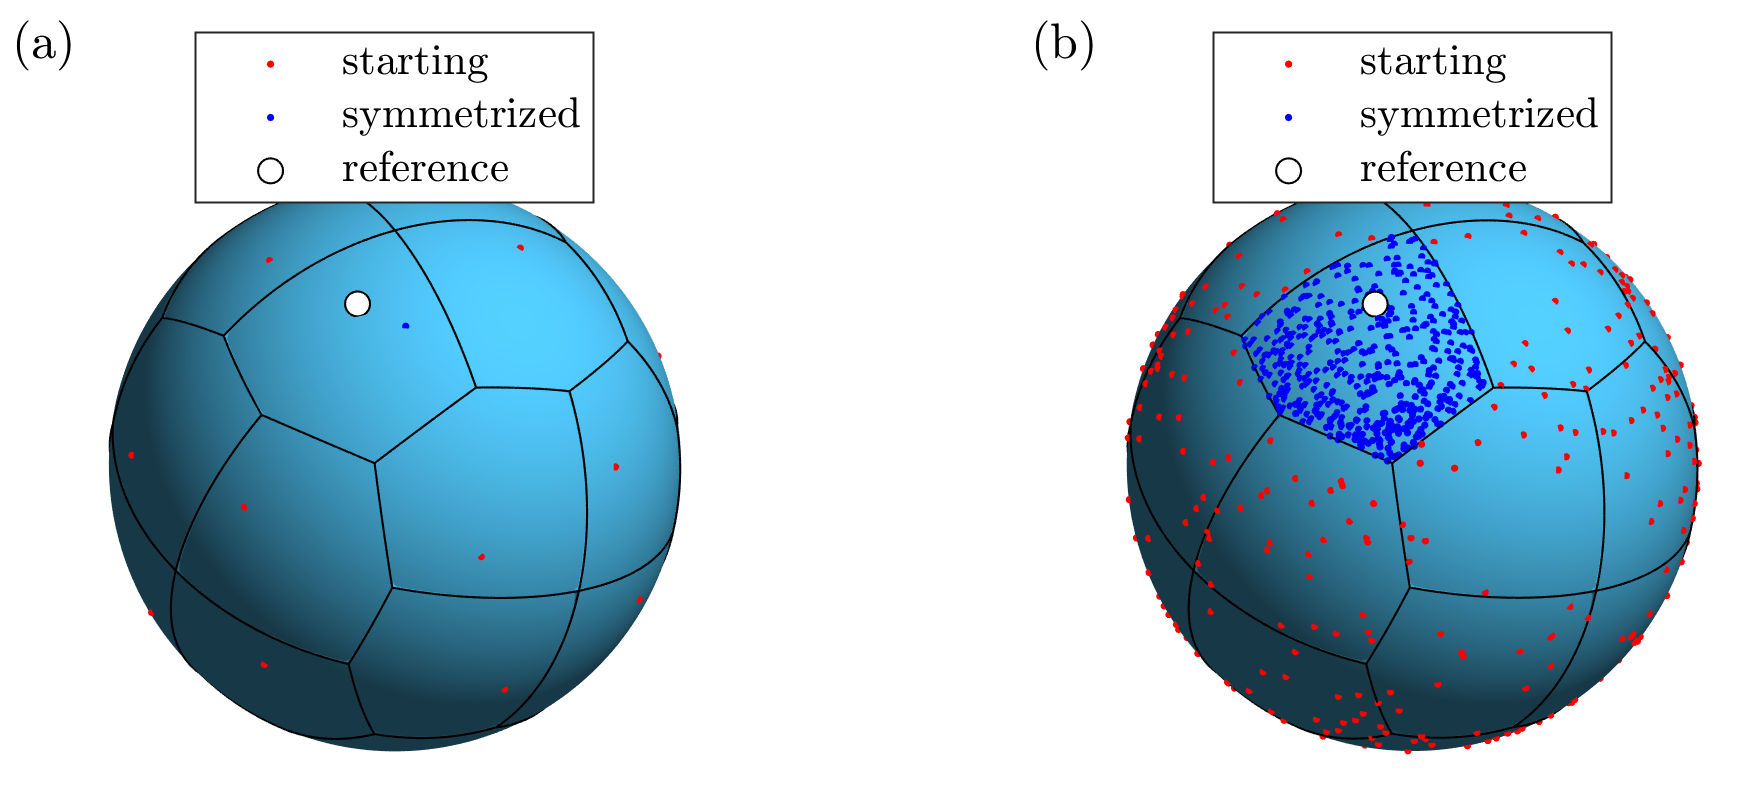
\includegraphics[scale=1]{voronoi.png}
    \caption{(a) 3D Cartesian analogue to a non-degenerate 7D Cartesian representation of U(1)-symmetrized \glspl{gbo} and \glspl{vfzo} (\glspl{vfzo} are inherently U(1)-symmetrized) which demonstrates the symmetrization of many points relative to a fixed, reference point (\refpt{}). This produces a 3D Cartesian \gls{vfz} point set (\sympt{}). (b) To further illustrate, a single input point (\singlept{}) is symmetrized (\singlesympt{}) relative to a fixed, reference point (\refpt{}) demonstrating that only one symmetrized point is found within the borders (\vbordercolor{}) of each of the Voronoi cells (\vcellcolor{}). The Voronoi tessellation is defined by the symmetric images of the reference point, and the spherical Voronoi diagram for this illustration is constructed using a modified version of \cite{luongVoronoiSphere2020}.}
    \label{fig:voronoi}
\end{figure*}

To calculate the distance between a given octonion, and the reference octonion, we employ the standard 8D Euclidean distance
\begin{equation}
    \label{eq:8Deuclidean_dist}
    d_{\text{E}}\!\left(o_{A},o_{B}\right) = {\left(\sum_{k=1}^{8} {\left(o_{A,k} - o_{B,k}\right)}^2 \right)}^{1/2}
    %why not just
    %\lVert o_A-o_B \rVert
\end{equation}
where $o_{X,k}$ is the $k$-the element of octonion $o_X$, and $o_X$ is normalized. Euclidean distance is an approximation to the true geodesic arc length on $\mathbb{S}^7$, which is given by
\begin{equation}
    \label{eq:7sphere_arc_length}
    d_{\text{S}}\!\left(o_{A},o_{B}\right)=\cos ^{-1}\left(o_A\cdot o_B\right)
\end{equation}
where $\cdot$ is the dot product, $\cos ^{-1}$ is the inverse cosine operator, and $o_A$ and $o_B$ are each normalized. In \cite{francisGeodesicOctonionMetric2019}, the original octonion distance metric can be defined by
\begin{equation}
    \label{eq:omega}
    d_\Omega\!\left(o_{A},o_{B}\right) = 2\cos ^{-1}\left(o_A\cdot o_B\right)
\end{equation}
where $o_A$ and $o_B$ are each normalized, where $d_\Omega$ can be seen to be simply twice the geodesic arc length: $d_\Omega = 2 d_{\text{S}}$. The definition of $d_\Omega$ has certain aesthetic benefits in that it mirrors the definition of a misorientation angle, $\omega_{AB}$, between two crystal orientations in the quaternion parameterization: $\omega_{AB} = 2 \cos^{-1}{\left(q_A \cdot q_B\right)}$.

Our choice to use $d_{\text{E}}$ instead of $d_{\text{S}}$ or $d_\Omega$ is motivated by the fact that it enables the use of standard algorithms, for a variety of operations, that require or assume Euclidean distances. In addition to enabling us to leverage the machinery of efficient and established algorithms, this choice can be justified by the following observations:
\begin{itemize}
    \item The minimum Euclidean distance \gls{seo} will be the same as the minimum arc length distance \gls{seo} because $d_{\text{S}}$ is a monotonically increasing function of $d_{\text{E}}$, for $d_{\text{S}}\!\left(d_{\text{E}}\right)\in[0,\pi]$ (\cref{fig:dist-parity}). 
    \item For the FCC point group symmetry ($m\bar{3}m$) the portion of $\mathbb{S}^7$ subtended by the \gls{vfz} is sufficiently small that the approximation $d_{\text{E}} \simeq d_{\text{S}}$ holds to very high accuracy\footnote{This is true when calculating the actual distance between two points in the \gls{vfz} without regard to symmetric images. When calculating the minimum distance between \glspl{seo} of two points, there are additional considerations that must be attended to as discussed in detail in \cref{sec:methods:vfz-dist}.} as shown in \cref{fig:dist-parity}. 
    \item Calculation of $d_{\text{E}}$ does not require the use of any inverse trigonometric functions and is about \SI{23}{\percent} faster than calculation of $d_{\text{S}}$ or $d_\Omega$.
\end{itemize}
% The expectation that a single, unique \gls{seo} will be found (within numerical tolerance and given a low-symmetry reference \gls{gbo}) is verified by several manual tests and internally within the symmetrization sub-routine \texttt{get\_octpairs.m} \cite{bairdFiveDegreeofFreedom5DOF2020} that is part of the \texttt{interp5DOF.m} package. Similar numerical tests reveal that inappropriately selecting a high-symmetry reference \gls{gbo} results in many degenerate minimum distance \glspl{seo}, with the identity octonion ($\{1,0,0,0,0,0,0,0\}\in\mathbb{R}^8$) \cite{francisGeodesicOctonionMetric2019} giving the highest degeneracy.

\subsubsection{Mapping \glsfmtshortpl{gb} to the \glsentrytitlecase{vfz}{long}}
\label{sec:methods:proj}

% With the reference GB chosen, and consequently the vfz defined, explain that a GB is mapped into the vfz simply by finding among its \glspl{seo} the one that is closest to the reference GB.

As described above in the 3D analogy, with a reference \gls{gbo} chosen ($o_{\text{ref}}$), and consequently the \gls{vfz} defined (\cref{sec:methods:framework:vfz}), a \gls{gbo} is mapped into the \gls{vfz} by finding among its \glspl{seo} the one that is closest to $o_{\text{ref}}$ according to $d_{\text{E}}$ (\cref{eq:8Deuclidean_dist}). This is performed for all \inpt{} and \outpt{} points with respect to $o_{\text{ref}}$, and the result is a \gls{vfz} point set.

% In the \gls{vfzo} framework, \glspl{seo} are chosen based on minimum Euclidean distance relative to a fixed, arbitrary reference octonion rather than allowing either octonion in a pair to vary in the traditional octonion approach with arc-length distances \cite{francisGeodesicOctonionMetric2019}. We consider all symmetrically equivalent \glspl{gbo} rather than a subset. For barycentric interpolation (\cref{sec:methods:bary}), we also remove a degenerate dimension via a rigid \gls{svd} transformation to 7D Cartesian and employ a further projection to 6D Cartesian only for the triangulation. These differences are summarized in Table \cref{tab:closed-mesh-comparison}. By choosing \glspl{seo} based on Euclidean distance with respect to a fixed octonion, a "closed-mesh" is obtained in the sense that directly computed Euclidean and arc length distances become meaningful and a unique octonion is found within numerical tolerance as long as the reference \gls{gbo} is low-symmetry (very likely based on random sampling and can be verified). This facilitates the use of standard triangulation and interpolation routines rather than needing to rely on pairwise-distance matrices where each distance calculation requires consideration of \glspl{seo}.

% \subsubsection{Generating Random \glsentrytitlecase{vfzo}{long}s} \label{sec:methods:rand} First, random \glspl{gbo} are formed by taking a random, cubochorically sampled quaternion \cite{singhOrientationSamplingDictionarybased2016} \texttt{qm} and random \gls{bp} unit vector \texttt{nA} pair and converting these to an octonion representation \texttt{o} using a modified version \cite{bairdFiveDegreeofFreedom5DOF2020} of \texttt{GBfive2oct.m} \cite{chesserGBOctonionCode2019} via \texttt{o=GBfive2oct(qm,nA)}. The conventions used for \texttt{qm} and \texttt{nA} are given in \cref{sec:intro:interp-error}. After mapping random \glspl{gbo} (\cref{sec:methods:rand}) into the \gls{vfz} (\cref{sec:methods:proj}) to obtain \glspl{vfzo} %

\subsubsection{Distance Calculations in the \glsentrytitlecase{vfz}{long}}
\label{sec:methods:vfz-dist}

% Explain how to compute distances in the vfz, and why you can now just use euclidean distances.
Euclidean distances are an accurate approximation of arc length distances in a \gls{vfz} because the difference between the two metrics for the maximum pairwise distance ($pd_{max} \simeq \SI{60}{\degree}$) in a \gls{vfz} is small as shown in \cref{fig:dist-parity}. However, when compared with the traditional octonion distance \cite{francisGeodesicOctonionMetric2019}, due to the presence of low-symmetry \glspl{gb} near the exterior of a \gls{vfz}, some \gls{gb} pairs will exhibit larger Euclidean or arc length distances than is truly representative (\cref{fig:dist-ensemble-k1-2-10-20}a). In other words, moving "past" the low-symmetry border of a \gls{vfz} will result in an instantaneous relocation to a possibly distant point in the \gls{vfz} that in reality is highly correlated. \Gls{vfzo} Euclidean, hyperspherical arc length, and octonion distances are computed via \vfzorepo{} function \texttt{\distfn{}.m} which is used in the symmetrization function \texttt{get\_octpairs.m}.

This is a limitation of the \gls{vfzo} framework which generates a \gls{vfz} with low-symmetry \glspl{gb} at the borders in contrast to typical \glspl{fz} \cite{patalaSymmetriesRepresentationGrain2013,homerGrainBoundaryPlane2015}. While defining a \gls{fz} with high-symmetry \glspl{gb} at the borders (especially mirror-symmetry \glspl{gb}) will certainly increase interpolation accuracy, the favorable interpolation results presented in this work are obtained because overestimation is infrequent within a small correlation length (e.g. \SI{10}{\degree} \cite{olmstedSurveyComputedGrain2009}, for which many \glspl{nn} fall within for a \num{50000} \gls{vfzo} set, see \cref{fig:nnhist-knn-50000}b), and underestimation is non-existent within numerical precision.

Overestimation imposes an arbitrary "sparseness" of data within a local region of influence common to the interpolation methods in this work, whereas underestimation would give erroneous high correlations between uncorrelated \glspl{gb}. Because only overestimation relative to traditional octonion distances exist in this work (\cref{fig:dist-ensemble-k1-2-10-20}), it is expected that large errors will occur infrequently, as shown in \cref{fig:brkparity50000}, and that overall errors will remain low as shown in \cref{fig:brkerror}, and \cref{tab:rmse-error-comparison,tab:mae-error-comparison}. 

While distance calculations are subject to these infrequent overestimates, they are largely immaterial for interpolation. This is because all of the interpolation methods in this work involve a region of influence that is small, so that if the distance to a \gls{nn} is overestimated it simply does not contribute to the interpolation. Consequently the accuracy of the interpolation is not significantly impacted by infrequent distance overestimates, and excellent results can be achieved without addressing this limitation. However, if even greater accuracy is desired it can be obtained for a relatively minor cost by considering multiple \glspl{vfz}.

We find that taking the minimum distance among several \gls{vfzo} sets defined by separate reference octonions leads to better correlation between the Euclidean approximation and the traditional octonion metric (\cref{fig:dist-ensemble-k1-2-10-20}). Additionally, \cref{fig:dist-ensemble-rmse-mae} shows that the error between scaled Euclidean distance and the traditional octonion metric decreases rapidly as the number of ensemble \gls{vfzo} sets increases. This confirms that employing a small ensemble of \gls{vfzo} sets results in significant improvement to the Euclidean distance approximation (\cref{fig:dist-ensemble-k1-2-10-20,fig:dist-ensemble-rmse-mae}) of the traditional octonion metric. However, as already mentioned, improvements to interpolation results are expected to be less significant since they are already robust to occasional distance overestimates.

%In our numerical tests, incorporating ensemble \gls{vfzo} sets with interpolation methods provides marginal increases of overall accuracy at some computational cost (e.g. approximately 10x using 10 ensembled \gls{vfzo} sets). We expect these modest overall accuracy improvements occur because \gls{gbe} predictions near the exterior of the \gls{vfz} where data may be arbitrarily sparse are improved.

\begin{figure*}
    \centering
    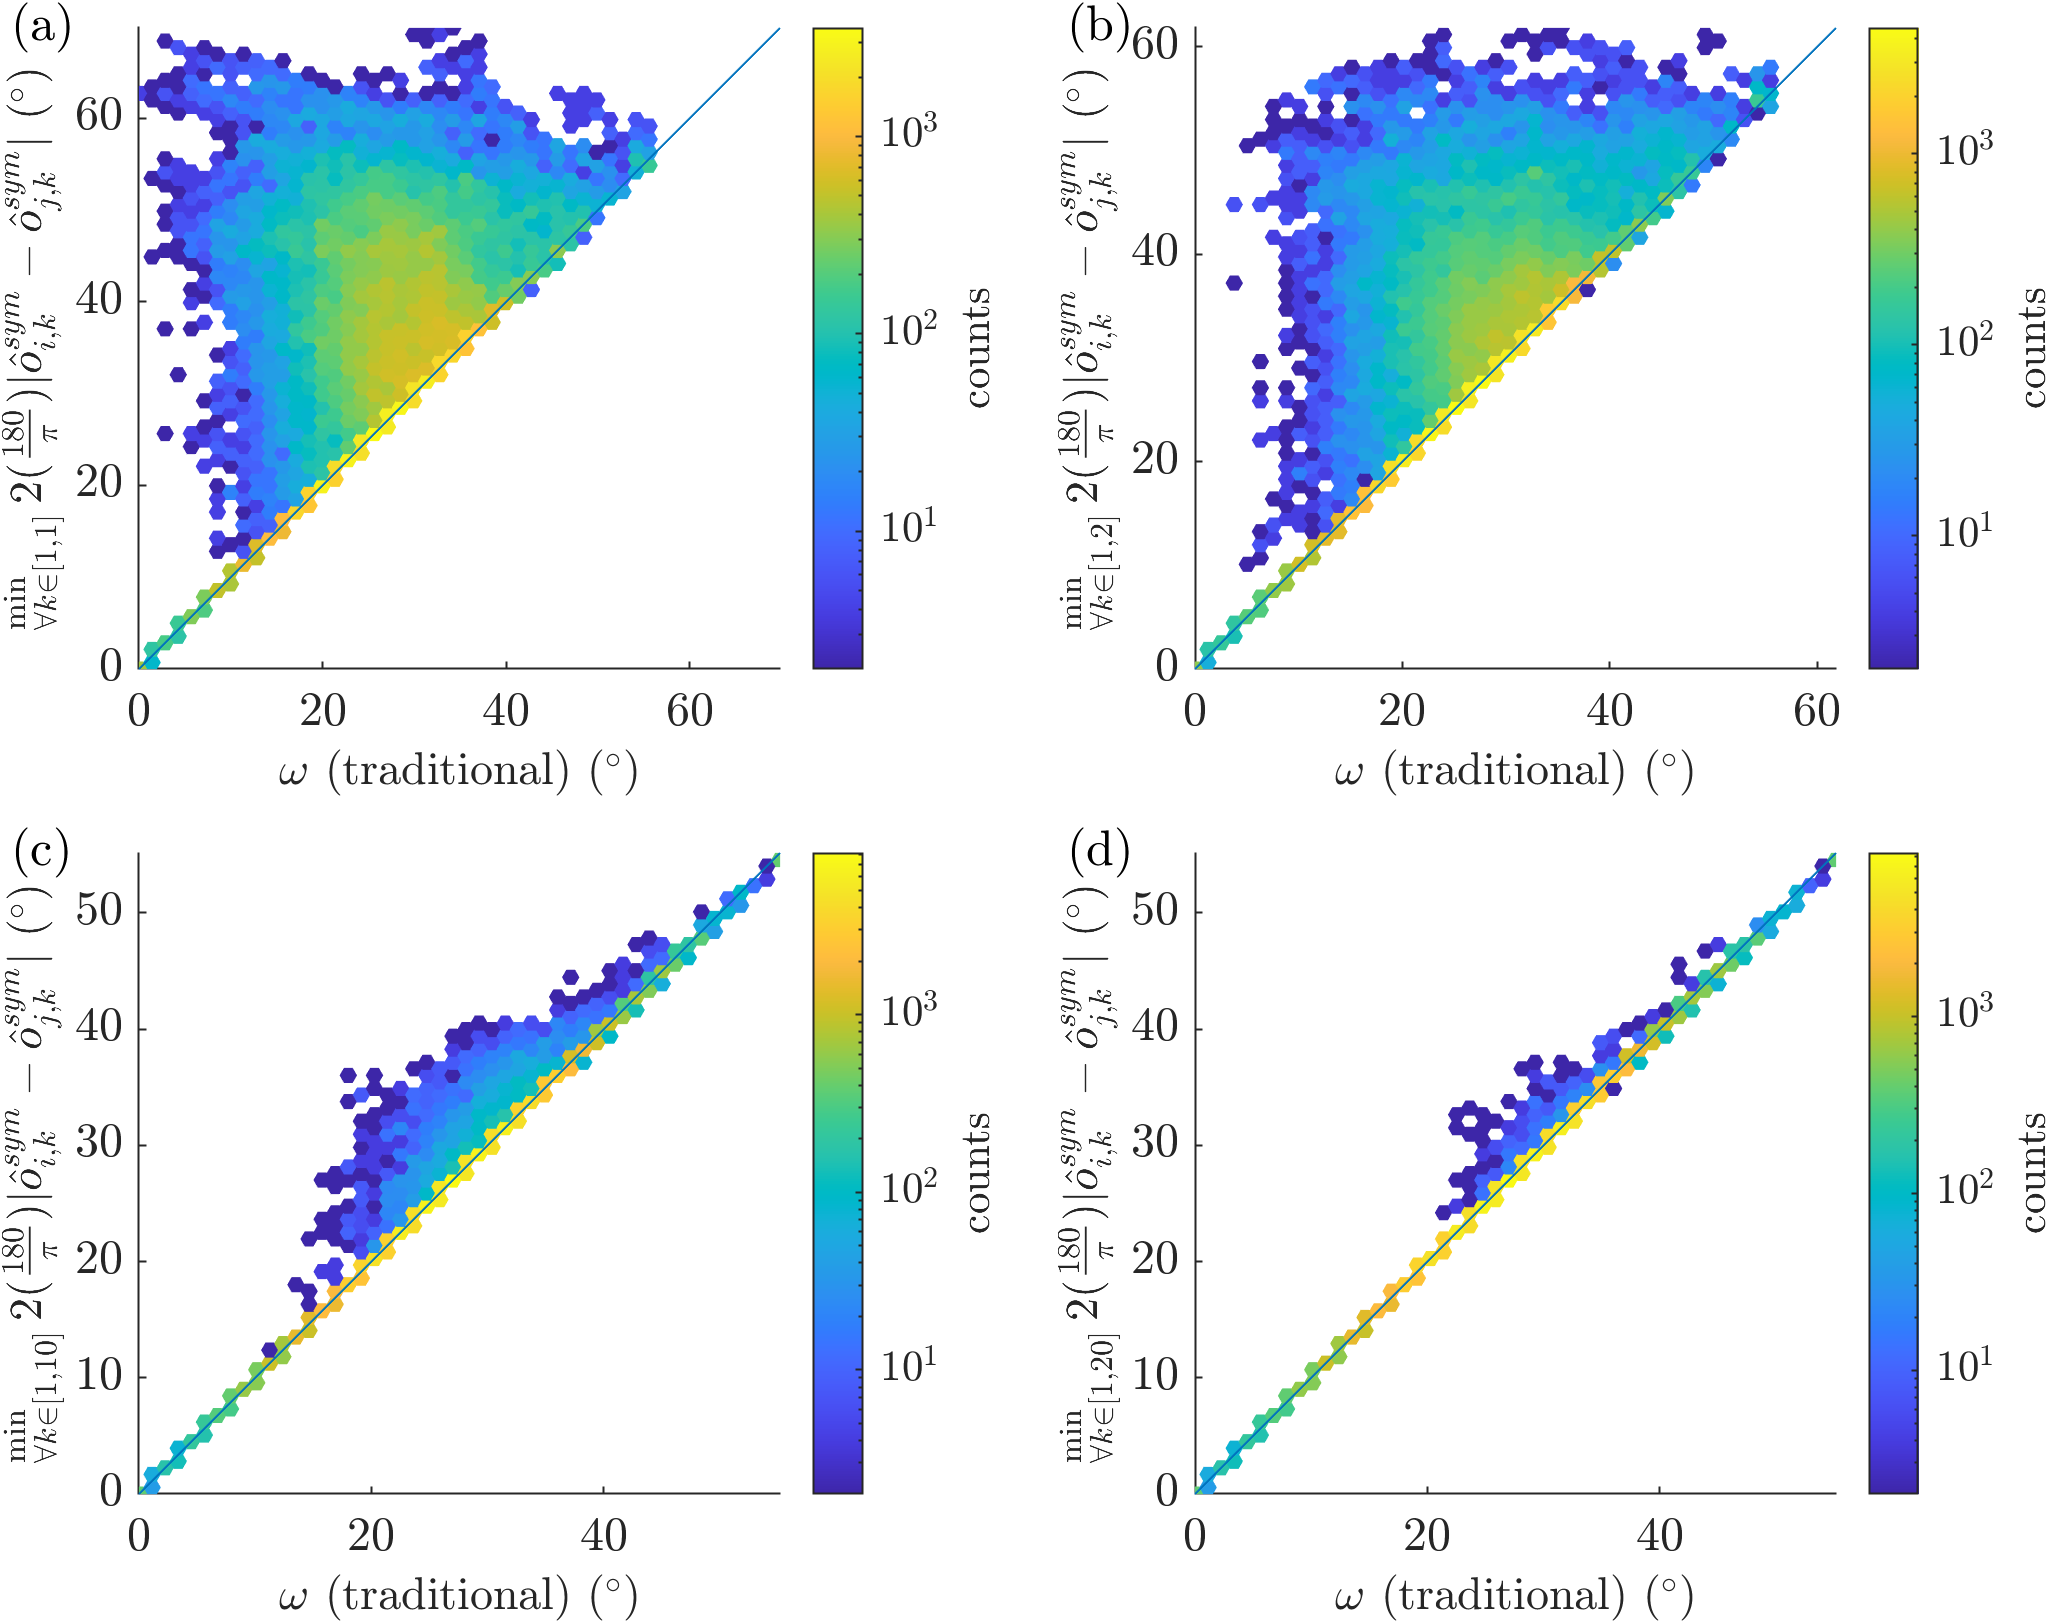
\includegraphics[scale=1]{figures/dist-ensemble-k1-2-10-20.png}
    \caption{Hexagonally binned parity plots of pairwise distances of 388 Ni bicrystals \cite{olmstedSurveyComputedGrain2009a}. Euclidean distance approximation is converted to octonions ($x_{i,j,k}=2\left(\frac{180}{\pi}\right)|\hat{o}_{i,k}^{\text{sym}}-\hat{o}_{j,k}^{\text{sym}}|$) for comparison with the traditional octonion metric \cite{chesserLearningGrainBoundary2020}. The minimum distance among an ensemble of \gls{vfzo} sets ($\min_{\forall k \in [1,k_{max}]}x_{i,j,k}$) is used for (a) 1, (b) 2, (c) 10, and (d) 20 \gls{vfzo} sets. As the number of \gls{vfzo} sets increases, the correlation between the Euclidean distance and the traditional octonion distance improves.}
    \label{fig:dist-ensemble-k1-2-10-20}
\end{figure*}

\begin{figure}
    \centering
    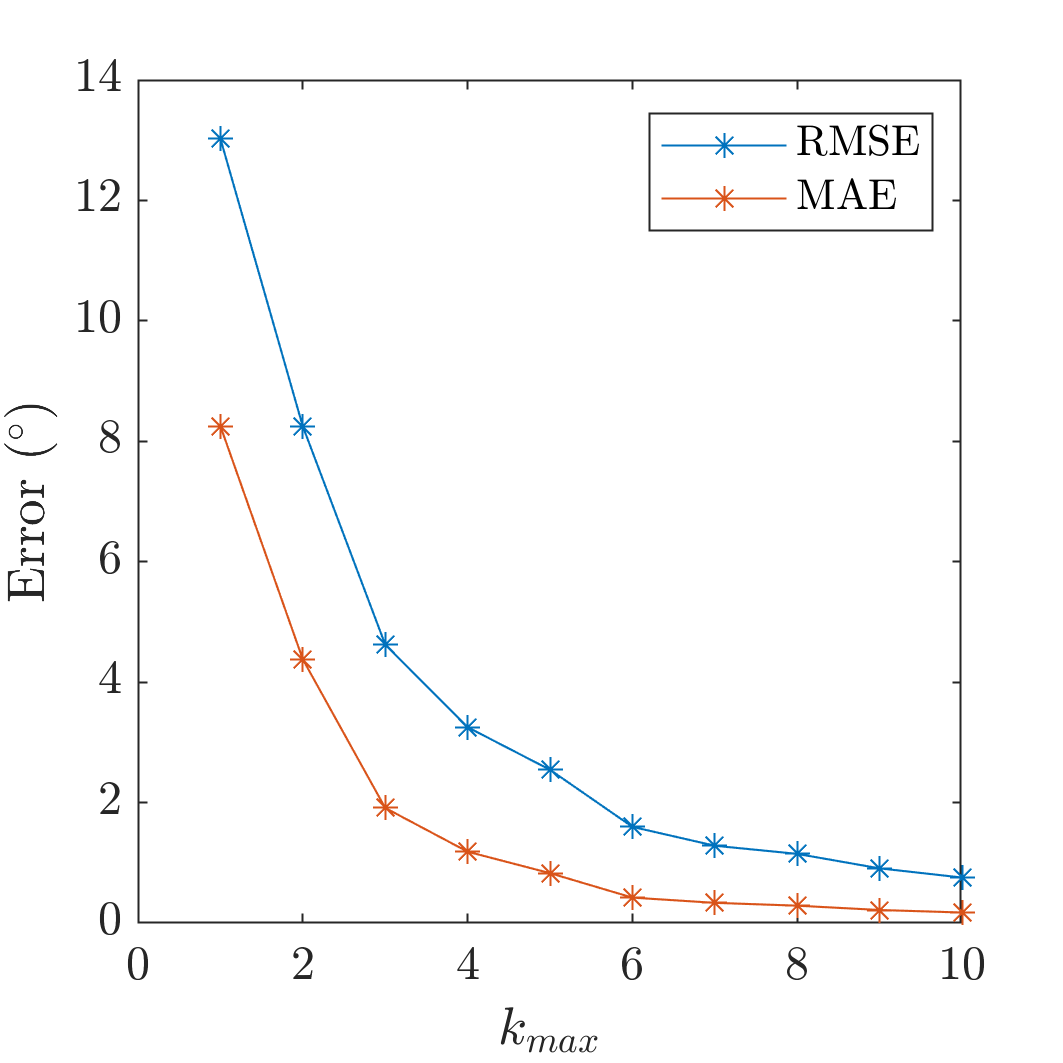
\includegraphics[scale=1]{figures/dist-ensemble-rmse-mae.png}
    \caption{\Gls{rmse} and \gls{mae} of pairwise distance errors for 388 Ni bicrystals \cite{olmstedSurveyComputedGrain2009a} of scaled Euclidean distance approximation relative to the traditional octonion metric \cite{chesserLearningGrainBoundary2020} (compare with \cref{fig:dist-ensemble-k1-2-10-20}). The minimum distance among an ensemble of \gls{vfzo} sets ($\min_{\forall k \in [1,k_{max}]}x_{i,j,k}$, where $x_{i,j,k}$ is the scaled Euclidean distance) is taken, iteratively adding consecutive sets up to $k_{max} = 20$. As the number of \gls{vfzo} sets increases, \gls{rmse} and \gls{mae} between the scaled Euclidean distance approximation and the traditional octonion distance decreases.}
    \label{fig:dist-ensemble-rmse-mae}
\end{figure}

\subsection{Generating Random \glsentrytitlecase{vfzo}{long}s}
\label{sec:methods:rand}
In addition to the 3 core operations of the \gls{vfzo} framework described in \cref{sec:methods:framework}, it will be necessary for our tests, and useful for other applications, to be able to generate points in the \gls{vfz}. We briefly explain here our process for accomplishing this. 

First, random \glspl{gbo} are formed by taking random misorientation quaternion (\texttt{qm}) and \gls{bp} normal (\texttt{nA}) pairs. Random misorientation quaternions are obtained via cubochoric sampling \cite{singhOrientationSamplingDictionarybased2016} (\texttt{get\_cubo.m}) and random \gls{bp} vectors are uniformly sampled in $\mathbb{R}^3 \in [-0.5,0.5]$ and normalized\footnote{Methods for uniform sampling of points on a sphere can be obtained by various methods described in \url{https://mathworld.wolfram.com/SpherePointPicking.html}, such as by normalizing a vector formed by random Gaussian variables}. After this, they are converted to \glspl{gbo} via \vfzorepo{} function \texttt{five2oct.m}. The \vfzorepo{} function \texttt{get\_five.m} returns the result of these several operations (see also \vfzorepo{} function \texttt{get\_ocubo.m} for generating random \glspl{gbo} directly).
%}a modified version \cite{bairdFiveDegreeofFreedom5DOF2020} of the original \texttt{GBfive2oct.m} function \cite{chesserGBOctonionCode2019} via

These (\texttt{qm},\texttt{nA}) pairs are then converted to an octonion representation, \texttt{o}, using \vfzorepo{ function \texttt{o=five2oct(qm,nA)} and symmetrized via \texttt{osym=get\_octpairs(o)}. A default reference octonion\footnote{This is generated by \texttt{get\_ocubo.m} using a random number generator seed of 10. We expect that \texttt{five2oct.m} combined with \texttt{get\_five.m} will generate near identical statistical properties to \texttt{get\_ocubo.m} which is supported by a visual comparison of pairwise distance histograms (not shown in this work).} is used for these calculations, unless specified by the user. The conventions used for \texttt{qm} and \texttt{nA} are given in \cref{sec:intro:interp-error}.

For the present work we use this procedure to generate random \gls{vfzo} sets containing between \num{100} to \num{50000} \glspl{vfzo}. The average \gls{nn} distance (over approximately 70 trials) of such sets ranges between \SI{10.7175 \pm 0.3684}{\degree} and \SI{2.6479 \pm 0.2254}{\degree}, respectively. \Cref{fig:nndist-vs-setsize} illustrates how the \gls{vfzo} average \gls{nn} distance varies with the cardinality of the set (i.e. number of random \glspl{vfzo} in the set). 

For a specific \num{50000} \gls{vfzo} set, the \gls{nn} octonion distance is \SI{\nnomega{}}{\degree} (\cref{fig:nnhist-knn-50000}a) while the average 100-th \gls{nn} distance is within \SI{10}{\degree} (\cref{fig:nnhist-knn-50000}b). This indicates that, on average, \outpt{} \glspl{vfzo} fall within a typical \gls{gb} correlation length (\SI{10}{\degree} \cite{olmstedSurveyComputedGrain2009}) of \inpt{} \glspl{vfzo} in large set sizes.
\begin{figure}
    \centering
    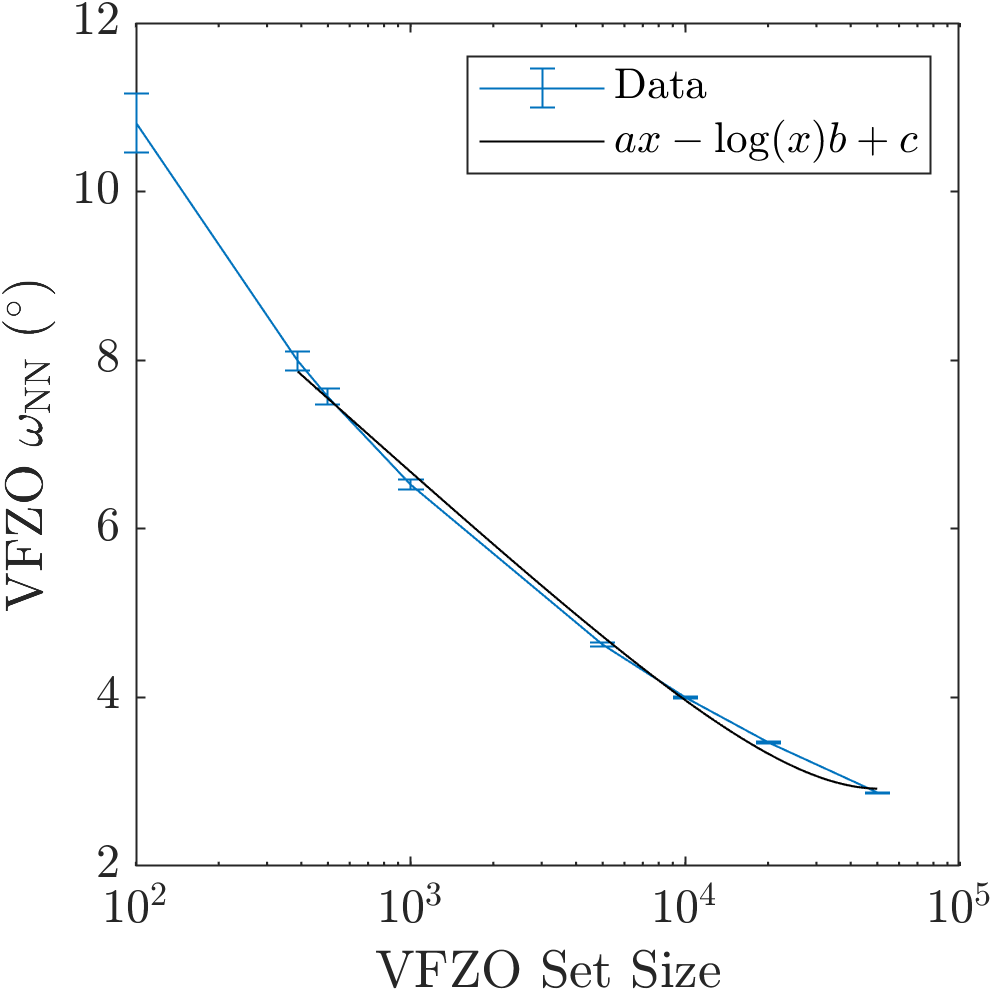
\includegraphics[scale=1]{nndist-vs-setsize.png}
    \caption{\Gls{nn} \gls{vfzo} ($\omega_{\text{NN}}$) distances ($^{\circ}$) versus \gls{vfzo} set size out of 70-80 random \gls{vfzo} sets per set size.}
    \label{fig:nndist-vs-setsize}
\end{figure}

\subsection{Interpolation in the \glsentrytitlecase{vfzo}{long} Framework}
\label{sec:methods:interp}

With the \gls{vfzo} framework established, it is possible to define interpolation schemes over the \gls{vfz} to predict the properties of new \glspl{gb} from the known properties of other \glspl{gb}. For one application of interest to us, it is necessary to evaluate multiple different functions over a fixed set of \inpt{} and \outpt{} \glspl{gbo}. In this section we first present a barycentric interpolation method that we have developed to efficiently accomplish this task by pre-computing the interpolation weights (which remain fixed only when the function being evaluated changes). We then present adaptations of three other interpolation methods (\gls{gpr}, \gls{idw}, and \gls{nn}) that are useful for other applications. We recommend the \gls{gpr} interpolation method for the \gls{vfzo} framework for most applications because it provides the best combination of accuracy and speed (\cref{sec:results}).

\subsubsection{Barycentric Interpolation}
\label{sec:methods:interp:bary}

% Give brief explanation of standard barycentric interpolation: you find which simplex the point is in, then you calculate the weights. The advantage of this approach is that the weight matrix only has to be computed once. If you interpolate different functions over the same query points, the weights don't change, so re-evaluation with a new function is rapid via a simple matrix multiplication.

% Explain how to adapt barycentric interpolation to the vfz: how to identify which simplex the query point falls in, and then how to compute the weights. Also explain and justify why you can use euclidean distances (i.e. because the vfz occupies a small portion of the 7-sphere it is nearly planar so euclidean distances and octonion distances are approximately equal and you can show tha figure here), and how that speeds things up.

Barycentric coordinates are a type of homogeneous coordinate system that reference a \outpt{} point within a simplex \cite{langerSphericalBarycentricCoordinates2006} or convex polytope \cite{floaterGeneralizedBarycentricCoordinates2015,meyerGeneralizedBarycentricCoordinates2002,langerSphericalBarycentricCoordinates2006} based on "masses" or weights at the vertices, which can be negative. The \outpt{} point is assumed to be the barycenter (center of mass) of the simplex or convex polytope, and weights at the vertices necessary to make this assumption true are determined. We utilize rigid \gls{svd} transformations and a standard triangulation algorithm (quickhull \cite{barberQuickhullAlgorithmConvex1996} via \texttt{delaunayn()} in \vfzorepo{} function \texttt{sphconvhulln.m}) to define a simplicial mesh (\cref{sec:app:bary:tri}). We then use barycentric weights (i.e. coordinates) for computing intersections of a point within a simplicial facet (\cref{sec:app:bary:int}) and for interpolation (\cref{sec:app:bary-interp}) \cite{langerSphericalBarycentricCoordinates2006}. A detailed explanation of the process is provided in \cref{sec:app}. The barycentric interpolation method is invoked in \texttt{interp5DOF.m} by setting the \texttt{method} argument to \texttt{'pbary'}.

\subsubsection{\glsentrytitlecase{gpr}{long}}
\label{sec:methods:interp:gpr}

% You don't need to give a detailed explanation of GPR, but you do need 1 sentence summarizing the idea and then point to REF for a general treatment. Explain any assumptions or adaptations that need to be done to use it with the vfz (e.g. presumably GPR is not actually operating on the surface of the 7-sphere, rather it is actually operating on all of $\mathbb{R}^8$, but because the vfz occupies a small portion of the 7-sphere it is nearly planar so euclidean distances and octonion distances are approximately equal, as mentioned previously, so it works without modification). Finally just explain that we used matlab's built-in \texttt{fitrgp()} function and the options used like you already have written.

\Gls{gpr} or Kriging uses the notion of similarity between points to fit Gaussian processes (random variables) to data based on prior information and provides uncertainty information in addition to interpolated or inferred values. For a general treatment of \gls{gpr}, see \cite{rasmussenGaussianProcessesMachine2006}. We use MATLAB's built-in function, \texttt{fitrgp()}, with all default parameters (MATLAB R2020b was used for the Fe simulation dataset, all other results employed MATLAB R2019b) except that \texttt{PredictMethod = 'fic'} was used regardless of the number of \inpt{} points, and we assume a Euclidean approximation of the \gls{vfz} (see \cref{sec:methods:vfz-dist} and \cref{fig:dist-parity}). A slower, more accurate, and more memory-intensive \texttt{PredictMethod = 'exact'} parameter choice is also available (\cref{sec:results:efficiency}). The \gls{gpr} interpolation method is invoked in \texttt{interp5DOF.m} by setting the \texttt{method} argument to \texttt{'gpr'}.

\subsubsection{\glsentrytitlecase{idw}{long} Interpolation}
\label{sec:methods:interp:idw}

% Explain the idea behind IDW in 1 sentence, then give the details of how you implemented it and any adaptations that are necessary for the present situation.

\Gls{idw} interpolation applies a weighted average to points within a neighborhood of a query point to obtain an interpolated value. \texttt{interp5DOF.m} implements a simple \gls{idw} approach based on \cite{tovarInverseDistanceWeight2020}. A default radius of influence of $r=\sqrt{2} \mu$ is used, where $\mu$ represents the mean \gls{nn} distance, and where octonion distance is approximated by the Euclidean distance or 2-norm (see \cref{sec:methods:vfz-dist}, and \cref{fig:dist-parity}). \gls{nn} interpolation (\cref{sec:methods:interp:nn}) is used for a given query point when there are no \inpt{} points in the radius of influence. The \gls{idw} interpolation method is invoked in \texttt{interp5DOF.m} by setting the \texttt{method} argument to \texttt{'idw'}.

\subsubsection{\glsentrytitlecase{nn}{long} Interpolation}
\label{sec:methods:interp:nn}

% Again, explain the idea in 1 sentence, and then give any special adaptations necessary.

\Gls{nn} interpolation takes the nearest \inpt{} point relative to a query point and assigns the value of the \gls{nn} \inpt{} point to the query point. This is implemented via the built-in MATLAB function \texttt{dsearchn()} using a Euclidean approximation of octonion distance (see \cref{sec:methods:vfz-dist}, and \cref{fig:dist-parity}). The \gls{nn} interpolation method is invoked in \texttt{interp5DOF.m} by setting the \texttt{method} argument to \texttt{'nn'}.

\section{Results and Discussion} \label{sec:results}

To illustrate the utility of the \gls{vfzo} framework for one application, namely interpolation, we compare the (i) accuracy (\cref{sec:results:accuracy}), and (ii) efficiency (\cref{sec:results:efficiency}) of the four previously described interpolation methods implemented over the \gls{vfz} with each other and with existing methods from the literature (see \cref{sec:intro}). We then demonstrate \gls{vfzo} \gls{gpr} interpolation applied to a large Fe bicrystal simulation dataset \cite{kimPhasefieldModeling3D2014} (\cref{sec:results:simulation}) which provides both \gls{gbe} and \gls{gbe} uncertainty predictions.

For these tests, we use the 5DOF GB energy function developed by Bulatov, Reed and Kumar \cite{bulatovGrainBoundaryEnergy2014} as a validation function which we refer to as the \gls{brk} function. For a given trial run, an \inpt{} \gls{vfzo} set, \texttt{o}, and a \outpt{} \gls{vfzo} set, \texttt{o2}, are randomly generated according to \cref{sec:methods:rand}. The validation function is evaluated at each of these points and the values are stored in the vectors \texttt{y} and \texttt{ytrue}, respectively. \texttt{o} and \texttt{o2} are \gls{svd} transformed together into a 7D Cartesian representation, which is an optional step for \gls{gpr}, \gls{nn}, and \gls{idw}, but not for barycentric interpolation. Finally, we use \texttt{interp5DOF.m} \cite{bairdFiveDegreeofFreedom5DOF2020} to predict the function value at the \outpt{} points, which are stored in the vector \texttt{ypred}. We repeat this process for each of the interpolation methods approximately 10 times per set size, and compare the predictions, \texttt{ypred}, to the true values, \texttt{ytrue}.

\begin{figure*}
\centering
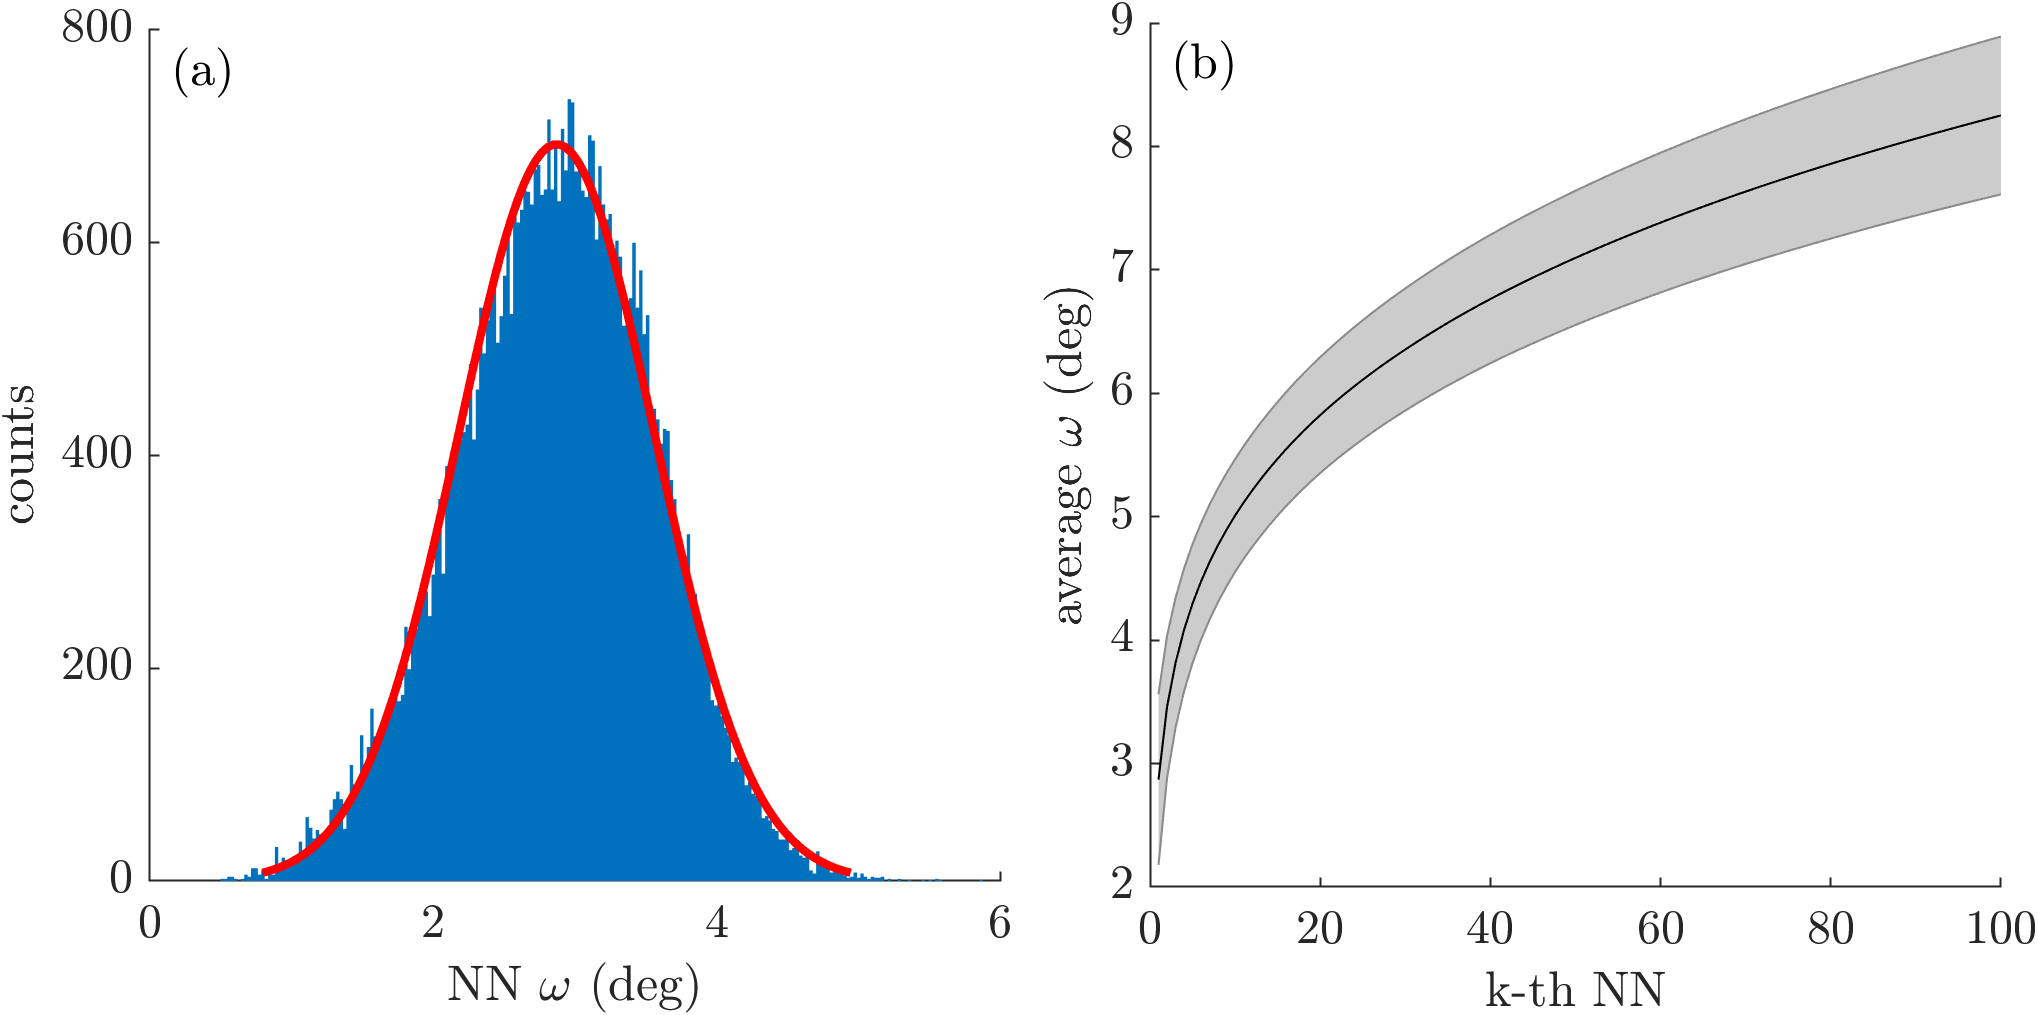
\includegraphics[scale=1]{nnhist-knn-50000.png}
\caption{Histogram of \gls{nn} octonion distances ($\omega$) in a \gls{vfzo} set of \num{50000} points (a). The average \gls{nn} distance was \SI{\nnomega}{\degree}. the average k-th nearest neighbor distances demonstrate many nearest neighbors fall within a tight tolerance (less then \SI{10}{\degree}) out of approximately 10 trial runs (b).}
\label{fig:nnhist-knn-50000}
\end{figure*}

\subsection{Interpolation Accuracy}
\label{sec:results:accuracy}

\Cref{fig:brkparity50000} provides hexagonally binned parity plots (via \vfzorepo{} function \texttt{parityplot.m} which depends on a modified version of \cite{beanHexscatter2020}) for each of the four interpolation methods.
\begin{figure*}
    \centering
    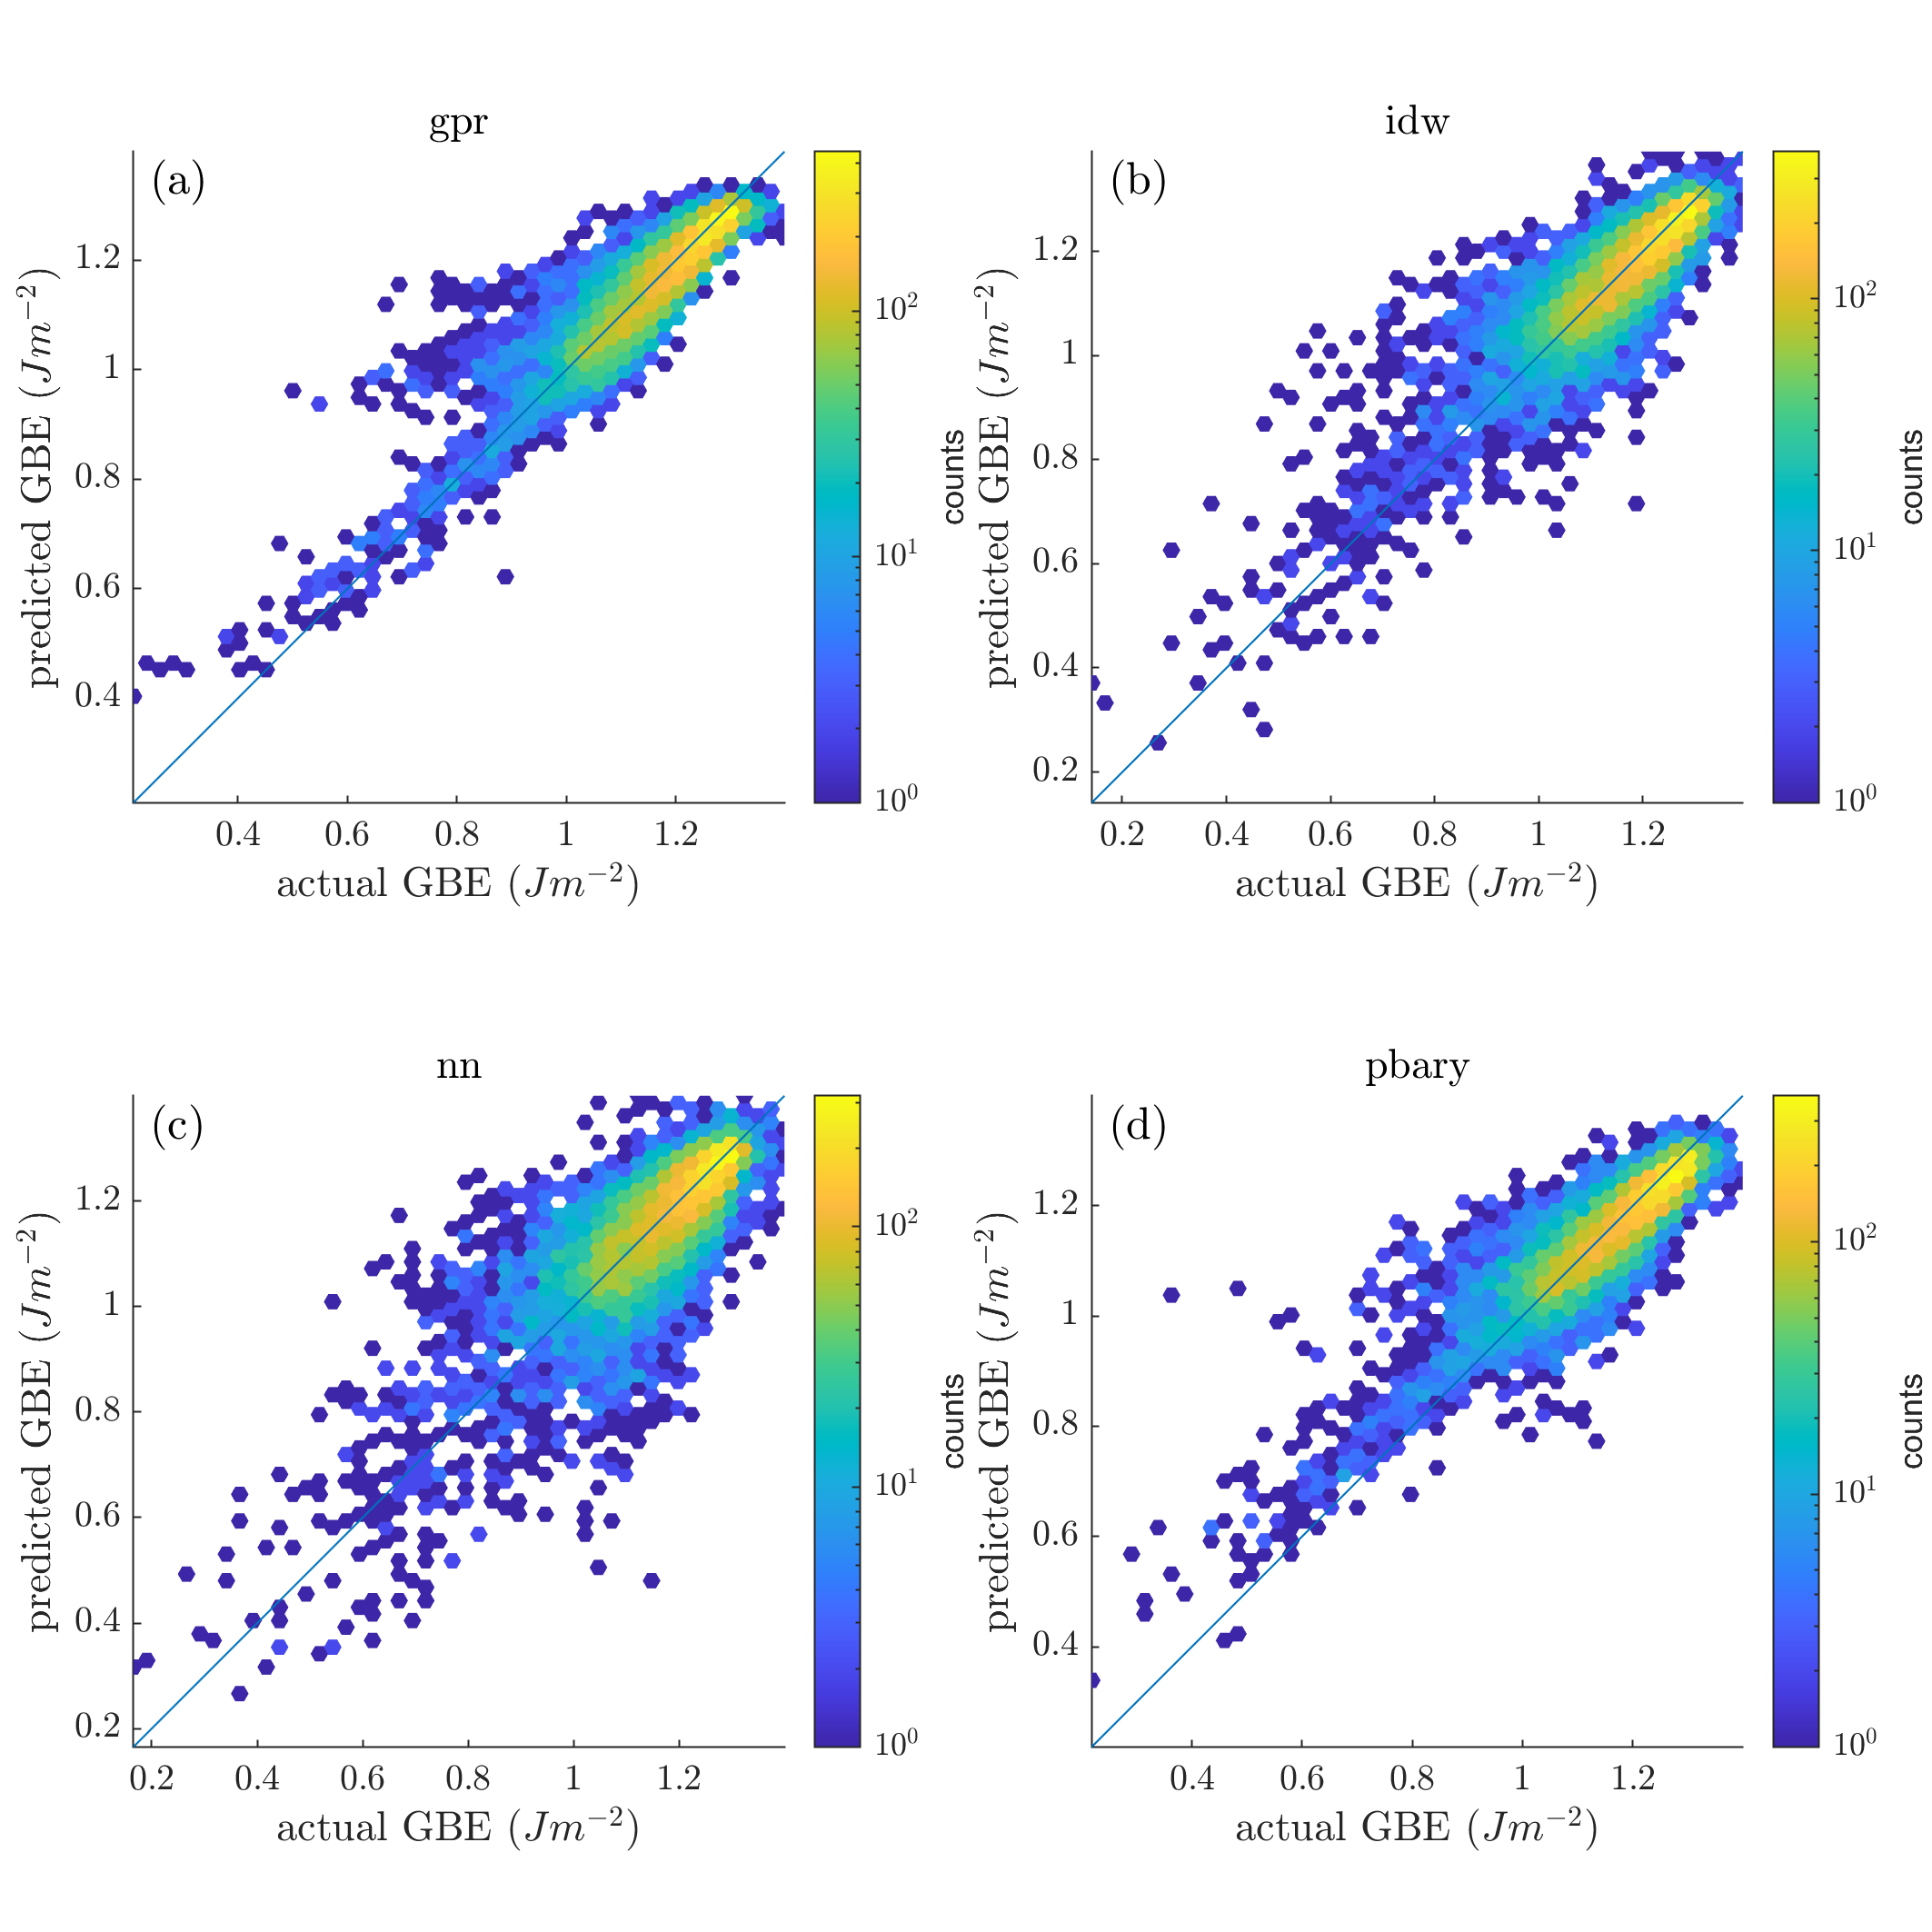
\includegraphics[scale=1]{brkparity50000.png}
    \caption{Hexagonally binned parity plots for \num{50000} \inpt{} and \num{10000} \outpt{} octonions formed via pairs of a random cubochorically sampled quaternion and a spherically sampled random boundary plane normal. Interpolation via (a) \gls{gpr}, (b) \gls{idw}, (c) \gls{nn}, and (d) barycentric coordinates.  \gls{brk} \gls{gbe} function for \gls{fcc} Ni \cite{bulatovGrainBoundaryEnergy2014} was used as the test function.}
    \label{fig:brkparity50000}
\end{figure*}

All of the methods permit successful interpolation, and the highest density region in all cases falls squarely on the parity line. The \gls{gpr} and barycentric results show a slight asymmetry such that low energy values are overpredicted more often than they are underpredicted. The width of the point clouds provides a qualitative indication of the dispersion in the prediction errors, and the color indicates the frequency of errors of a given magnitude. As can be seen, the vast majority of errors are very small (the highest density---yellow region---is concentrated on the line of parity). Quantitative measures of the overall accuracy are presented for \gls{rmse} (\cref{tab:rmse-error-comparison}) and \gls{mae} (\cref{tab:mae-error-comparison}) along with results of prior work where available. Error metrics are obtained via \vfzorepo{} function \texttt{get\_errmetrics.m}.

% Please add the following required packages to your document preamble:
% \usepackage{booktabs}
\begin{table*}
\centering
\caption{Comparison of average interpolation \gls{mae} (approximately 10 trial runs) for each interpolation method in the present work, using \num{50000} points in the definition of the \gls{vfz}. Comparison to the work of other authors is also included. A constant model (Cst, Avg \gls{mae}), whose value was chosen to be the mean of the \inpt{} \gls{gbe} was used as a control. The last two columns represent the reduction ($\downarrow$) in \gls{mae} in absolute units of \SI{}{\J\per\square\meter} and \% relative to the control model, respectively.}
\label{tab:mae-error-comparison}
\begin{tabular}{@{}llllll@{}}
\toprule
Method &
  \# \glspl{gb} &
  \thead{\gls{mae} \\   (\SI{}{\J\per\square\meter})} &
  \thead{Cst, Avg \gls{mae} \\   (\SI{}{\J\per\square\meter})} &
  \thead{\gls{mae} $\downarrow$ \\   (\SI{}{\J\per\square\meter})} &
  \thead{\gls{mae}   $\downarrow$ \\ (\%)} \\ \midrule
\Gls{gpr}                                            & \num{50000} & \num{0.0145} & \num{0.0955} & \num{0.081}  & \num{84.8} \\
Barycentric                                          & \num{50000} & \num{0.0145} & \num{0.0955} & \num{0.081}  & \num{84.8} \\
\gls{idw}                                            & \num{50000} & \num{0.0225} & \num{0.0955} & \num{0.073}  & \num{76.4} \\
\gls{nn}                                             & \num{50000} & \num{0.0307} & \num{0.0955} & \num{0.0648} & \num{67.9} \\
\gls{ann}   \cite{restrepoUsingArtificialNeural2014} & \num{17176} & \num{0.0486} & \num{0.0617} & \num{0.0131} & \num{21.2} \\
\gls{lkr}   \cite{chesserLearningGrainBoundary2020}  & \num{388}   & \num{0.0977} & \num{0.1752} & \num{0.0775} & \num{44.2} \\ \bottomrule
\end{tabular}
\end{table*}

%, except in the case of \gls{lobpcg} which used the mean of the true \gls{gbe} values instead. Additionally, \gls{lobpcg}$^*$ is not interpolation, but rather a complementary technique of reconstruction of specific \glspl{gbe} using polycrystalline data. 

% Please add the following required packages to your document preamble:
% \usepackage{booktabs}
\begin{table*}
\centering
\caption{Comparison of average interpolation \gls{rmse} (approximately 10 trial runs) for each interpolation method in the present work, using \num{50000} points in the definition of the \gls{vfz}. Comparison to the work of other authors is also included. A constant model (Cst, Avg \gls{rmse}), whose value was chosen to be the mean of the \inpt{} \gls{gbe} was used as a control. The last two columns, \gls{rmse} $\downarrow$ (\SI{}{\J\per\square\meter} and \gls{rmse}   $\downarrow$ (\%)), represent the reduction in \gls{rmse} in units of \SI{}{\J\per\square\meter} and \% relative to the control model, respectively.}
\label{tab:rmse-error-comparison}
\begin{tabular}{@{}llllll@{}}
\toprule
Method &
  \thead{\# \glspl{gb}} &
  \thead{\gls{rmse} \\   (\SI{}{\J\per\square\meter})} &
  \thead{Cst, Avg \gls{rmse} \\   (\SI{}{\J\per\square\meter})} &
  \thead{\gls{rmse} $\downarrow$ \\   (\SI{}{\J\per\square\meter})} &
  \thead{\gls{rmse}   $\downarrow$ \\ (\%)} \\ \midrule
\Gls{gpr}                                            & \num{50000} & \num{0.0218} & \num{0.1283} & \num{0.1065} & \num{83}   \\
Barycentric                                          & \num{50000} & \num{0.0238} & \num{0.1283} & \num{0.1045} & \num{81.4} \\
\gls{idw}                                            & \num{50000} & \num{0.0356} & \num{0.1283} & \num{0.0927} & \num{72.3} \\
\gls{nn}                                             & \num{50000} & \num{0.0445} & \num{0.1283} & \num{0.0838} & \num{65.3} \\
\gls{ann}   \cite{restrepoUsingArtificialNeural2014} & \num{17176} & \NA          & \num{0.0854} & \NA          & \NA        \\
\gls{lkr}   \cite{chesserLearningGrainBoundary2020}  & \num{388}   & \num{0.0977} & \num{0.2243} & \num{0.1266} & \num{56.4} \\ \bottomrule
\end{tabular}
\end{table*}

%, except in the case of \gls{lobpcg}$^*$ which used the mean of the true \gls{gbe} values instead. Additionally, \gls{lobpcg} is not interpolation, but rather a complementary technique of reconstruction of specific \glspl{gbe} using polycrystalline data.

% \begin{table}
% \caption{Comparison of average runtime for each interpolation method in the present work, using \num{50000} points in the definition of the \gls{vfz}. Comparison to the work of other authors is also included. A constant model, whose value was chosen to be the mean of \texttt{f\_v}, was used as a control.}
% \centering
% \begin{tabular}{lccc}
% \toprule
% Method & \# \glspl{gb} & Runtime (\SI{}{seconds}) \\
% \midrule
% \Gls{gpr} & x & x \\
% Barycentric & x & x \\
% \gls{idw} & x & x \\
% \gls{nn} & x & x \\
% Constant & 0.13 & 0.097 \\
% LOBPCG \cite{shenDeterminingGrainBoundary2019} & 0.01--0.03 & --- \\
% ANN \cite{restrepoUsingArtificialNeural2014} & --- & 0.05--0.09 \\
% LKR \cite{chesserLearningGrainBoundary2020} & 0.0977 & --- \\
% \bottomrule
% \end{tabular}
% \label{tab:runtime-comparison}
% \end{table}

To aid in objective interpretation of the error metrics, comparison is made to a constant valued control model, whose value is chosen to be the average of \texttt{y} (approximately \SI{1.16}{\J\per\square\meter} in the limit of $\texttt{\inptvar{}} \rightarrow \infty$) resulting in \gls{rmse} and \gls{mae} values of approximately \num{\avgrmse{}} and \SI{\avgmae{}}{\J\per\square\meter}. Because the true models differed for other articles, equivalent errors obtained by a constant valued control model (mean of \inpt{} \gls{gbe} values) were also included for prior work in \cref{tab:rmse-error-comparison,tab:mae-error-comparison}. This comparison with the relevant constant-valued function gives a sense of the complexity and variability of the validation function employed in each work and allows for a more objective comparison between differing works. For example, the \gls{rmse} for the constant function compared to the validation function employed for the \gls{ann} interpolation method in \cite{restrepoUsingArtificialNeural2014} is \SI{0.0854}{\J\per\square\meter}; in contrast, the \gls{rmse} for the constant function compared to the BRK validation function used in this work is \SI{0.1302}{\J\per\square\meter} (see \cref{tab:rmse-error-comparison}). This suggests that the BRK validation function is more complex and therefore less well approximated by a constant than the validation function used to test the \gls{ann} interpolation method in \cite{restrepoUsingArtificialNeural2014}. Consequently, the improved performance of the present methods is even more notable in that the validation function employed here is more difficult to interpolate.

To give further context to the results of this and prior works, it is useful to consider what the intrinsic error is for typical GB property data. This provides an idea of the minimum possible interpolation error, since one cannot hope to have lower error in the interpolation than already exists in the input data itself. One such estimate is furnished by the work of \citet{shenDeterminingGrainBoundary2019}, who introduced a non-discretizing approach to extract relative \gls{gb} energies from polycrystalline samples using the \gls{lobpcg} method. Their approach utilizes regularization imposed on \gls{tj} equilibrium equations and \gls{knn} distances. Using \num{60000} \glspl{tj} (\num{180000} \glspl{gb}) and a custom, non-smooth validation function they obtained \gls{gbe} \gls{rmse} values of \SI{0.0076}{\J\per\square\meter} and \SI{0.0277}{\J\per\square\meter} for \gls{gbe} values greater than \SI{0.9}{\J\per\square\meter} and less than \SI{0.9}{\J\per\square\meter}, respectively. This suggests that an optimistic estimate for the error in \emph{experimental} \gls{gbe} data obtained using such a method is on the order of \SIrange{0.0076}{0.0277}{\J\per\square\meter}, which also serves as an estimate of the minimum achievable interpolation error for any of the interpolation methods described here. Similar analysis for \emph{simulation} data is provided in \cref{sec:results:simulation}. Again comparing a constant-valued control model\footnote{We use the mean of the true \glspl{gbe} from their validation function to define the constant-valued control model.} to the validation function they used, we calculate a \gls{rmse} and \gls{mae} of \SIlist{0.0976;0.0466}{\joule\per\square\meter}, respectively. This implies that the validation model used by \citet{shenDeterminingGrainBoundary2019} is simpler\footnote{\citet{shenDeterminingGrainBoundary2019} used 8 cusps of varying depths and widths based on the Read-Shockley model and unity \gls{gbe} everywhere else.} than the \gls{brk} validation model employed in the present work.

As shown in \cref{tab:mae-error-comparison,tab:rmse-error-comparison}, of the four interpolation methods from this work, \Gls{gpr} has the lowest error, both in terms of \gls{rmse} and \gls{mae}, while \gls{nn} has the highest error. Compared to a constant valued control model, \gls{gpr} interpolation reduced the prediction \gls{rmse} by \SI{\gprrmsePercReduction}{\percent}, which outperforms all of the interpolation methods in this work with respect to accuracy, as well as those considered from the literature. After \gls{gpr} the next most accurate methods are barycentric and \gls{lkr} interpolation (with the order depending on whether \gls{rmse} or \gls{mae} are used as the error measure), followed by \gls{idw}, \gls{nn} and then \gls{ann}. It is worth noting that the \gls{rmse} interpolation error for the \gls{gpr} and barycentric methods is comparable to the minimum achievable interpolation error (the estimated error in experimental data obtained via the \gls{lobpcg} analysis mentioned previously). This is even more significant because the \gls{brk} validation function used in the present work is more complex and difficult to interpolate than that used in \cite{shenDeterminingGrainBoundary2019}.

The accuracy of the predictions made using the \gls{vfz} methods depends on the \gls{vfzo} set size and distribution. % resolution of the \gls{vfzo} set.
\Cref{fig:brkerror} compares the prediction accuracy for each of the 4 methods to the constant valued control model, as a function of the number of \inpt{} \glspl{vfzo} (\texttt{\inptvar{}}). As expected, higher density \gls{vfzo} sets result in lower error, but eventually gives diminishing returns (\cref{fig:brkerror}). Moreover, the standard deviations produced via multiple runs are tightly constrained and generally shrink as the \gls{vfzo} set size increases. 

\Gls{gpr} consistently gives lower error than the other three interpolation methods for all \gls{vfzo} set sizes. 
%It is interesting to see that despite qualitative differences in the parity plots for barycentric and \gls{idw} interpolation, these two methods produce similar \gls{rmse} and \gls{mae} values.
\Gls{nn} interpolation produces the worst error of the four methods, but is better than a constant valued control model (i.e. average of the \inpt{} \glspl{gbe}) so long as \texttt{\inptvar{}} exceeds a few hundred \inpt{} points.

It is worthwhile to note that both \gls{gpr} and \gls{idw} are kernel-based in that a model parameter controls the size of the region that can influence the interpolation results. In the \gls{gpr} case, this is automatically calculated via an internal fitting routine of \texttt{fitrgp()}. \gls{nn} distance distributions (\cref{fig:nnhist-knn-50000}) can lead to insight about correlation lengths in a given \gls{vfzo} set and is used in the \gls{idw} implementation. For \gls{idw}, the radius of influence is set to $r=\sqrt{2} \mu$, where $\mu$ is the mean \gls{nn} distance. It is likely that better tuning of the kernel parameters in these two methods (such as use of built-in hyperparameter optimization in the case of \texttt{fitrgp()}) could further decrease their interpolation errors.

By contrast, barycentric interpolation automatically adjusts its effective region of influence because the size of the simplices in the mesh decreases as the number of vertices increases. More uniformly distributed meshes (such as obtained via constrained optimization \cite{dolanBenchmarkingOptimizationSoftware2004,ConstrainedElectrostaticNonlinear2020}) will likely result in lower, more uniform interpolation error, especially for this simplex-based approach which can exhibit high-aspect ratio facets and non-intersections outside the bounds of the mesh (\cref{fig:high-aspect-non-int}). While the barycentric interpolation error is always higher than \gls{gpr} for the considered set sizes, at \num{50000} \glspl{vfzo}, the errors of \gls{gpr} and barycentric interpolation are nearly identical. %( However, this may be computationally infeasible for large mesh sizes.

% While not implemented in this work, it is expected that an \gls{ann} such as in \cite{restrepoUsingArtificialNeural2014} could lead to even lower interpolation error than \gls{gpr} for large mesh sizes. % (e.g. https://www.mathworks.com/help/deeplearning/ref/narxnet.html, https://www.mathworks.com/help/deeplearning/function-approximation-and-nonlinear-regression.html)

\begin{figure*}
    \centering
    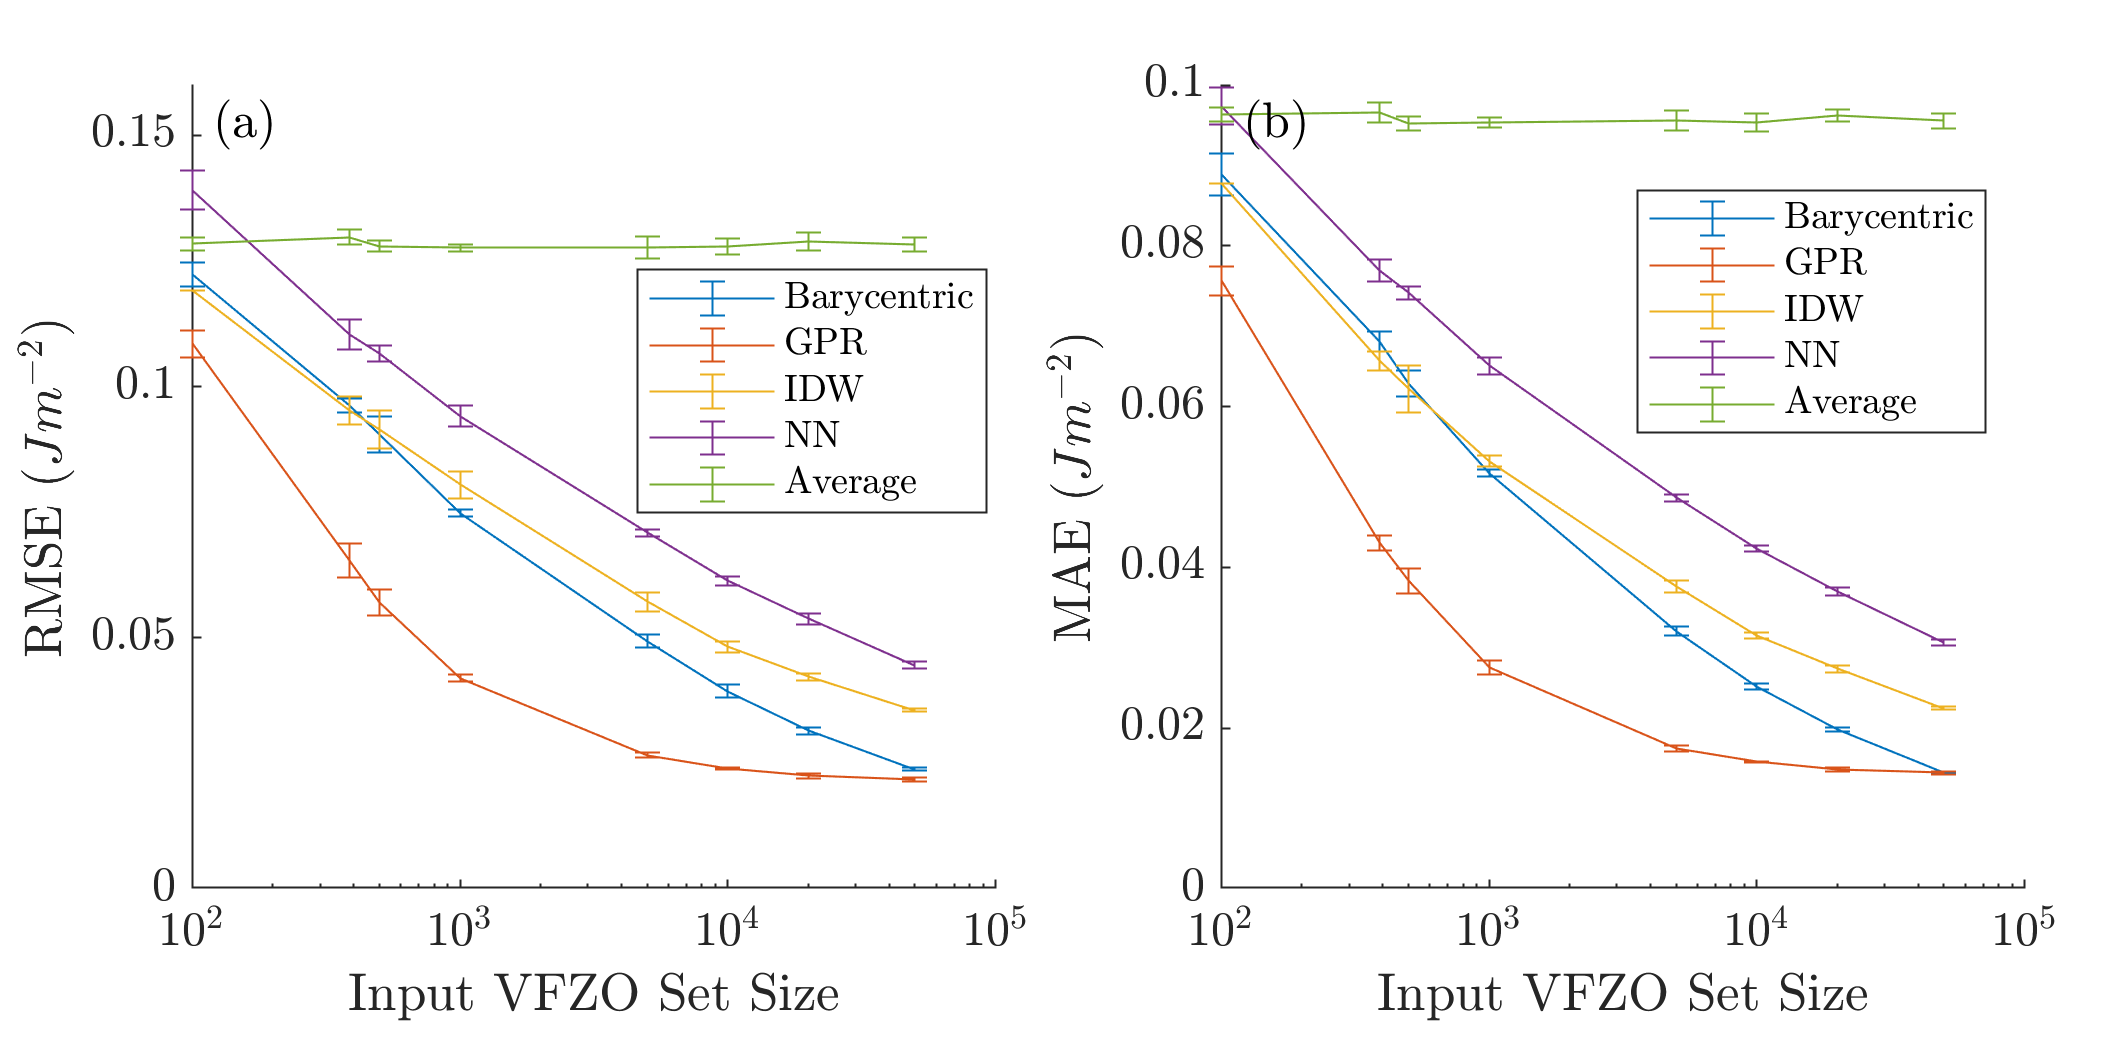
\includegraphics[scale=1]{brkerror.png}
    \caption{Average \gls{rmse} (a) and average \gls{mae} (b) vs. number of \inpt{} points for (planar) barycentric (blue), \gls{gpr} (orange), \gls{idw} (yellow), and \gls{nn} (purple) interpolation for approximately 10 random runs with different \inpt{} and \outpt{} points. Standard deviations of approximately 10 runs are also included. Compare with approximately \SI{\avgrmse{}}{\J\per\square\meter} and \SI{\avgmae{}}{\J\per\square\meter} \gls{rmse} and \gls{mae}, respectively, for a constant, average model (green) using the average of the \inpt{} properties (approximately \SI{1.16}{\J\per\square\meter}).}
    \label{fig:brkerror}
\end{figure*}

Predictions for each of the four interpolation methods are plotted as a function of distance along a 1D arc ($\overline{AB}$) between two \glspl{vfzo}, $A$ and $B$, as shown in \cref{fig:tunnel-50000}. Approximate coordinates for $A$ and $B$ are given in \cref{tab:tunnel-AB}, and each intermediate point between $A$ and $B$ resides on the surface of a hypersphere. Each model used its own set of \num{50000} random \inpt{} \glspl{vfzo} with \gls{gbe} sampled via the \gls{brk} validation function. The two \glspl{vfzo} were chosen by taking the furthest apart pair out of \num{20000} \glspl{vfzo} which thus approximates the largest dimension of the \gls{vfz} where each endpoint is close to the true \gls{vfz} exterior. We believe this is the first\footnote{\Gls{oslerp} results from \cite{francisGeodesicOctonionMetric2019} plots \gls{gb} \textit{structure} continuously between two \glspl{gb}, and \cite{chesserLearningGrainBoundary2020} performs cross-validation on the simulated Olmsted Ni \glspl{gb}. The results in both \cite{francisGeodesicOctonionMetric2019} and \cite{chesserLearningGrainBoundary2020} are distinct from what is presented here: a plot of continuously interpolated \glspl{gbe} between two \glspl{gb}.} plot of a \gls{gb} property continuously interpolated between two arbitrary \glspl{gb} (i.e. neither residing entirely in a single \gls{mfz} nor a single \gls{bpfz}). Such visualizations can naturally be extended to 2D and 3D by plotting colored points in a triangle or tetrahedron, respectively, all of which (1D, 2D, and 3D) represent small "slices" of the \gls{gb} character space. Such visualizations naturally suggest the ability to determine and verify numerical derivatives or gradients of \gls{gb} properties without being restricted to a \gls{gb} subspace (e.g. \gls{mfz} or \gls{bpfz}) which can be a useful mathematical construct for the \gls{gb} community. For example, steepest descent paths and all local \gls{gbe} minima can be found and used in grain growth simulations. In such a case, use of ensembled \gls{vfzo} interpolation may be necessary to prevent discontinuity artifacts when crossing the exterior of a \gls{vfz}.

% Please add the following required packages to your document preamble:
% \usepackage{booktabs}
\begin{table*}[]
\centering
\caption{Approximate coordinates of \glspl{vfzo} A and B used for the interpolation in \cref{fig:tunnel-50000}. Individual quaternions of each octonion are given in the active sense and in the laboratory reference frame with an assumed \gls{gb} normal pointing in the +z direction, also in the laboratory reference frame.}
\label{tab:tunnel-AB}
\begin{tabular}{@{}lllllllll@{}}
\toprule
Octonion & o(1)   & o(2)    & o(3)    & o(4)    & o(5)    & o(6)   & o(7)    & o(8)   \\ \midrule
A        & 0.8658 & -0.4269 & -0.1270 & 0.2280  & 0.2810  & 0.8390 & -0.3852 & 0.2622 \\
B        & 0.4684 & -0.7657 & -0.4100 & -0.1617 & -0.1483 & 0.8204 & -0.3588 & 0.4198 \\ \bottomrule
\end{tabular}
\end{table*}
    
\begin{figure}
    \centering
    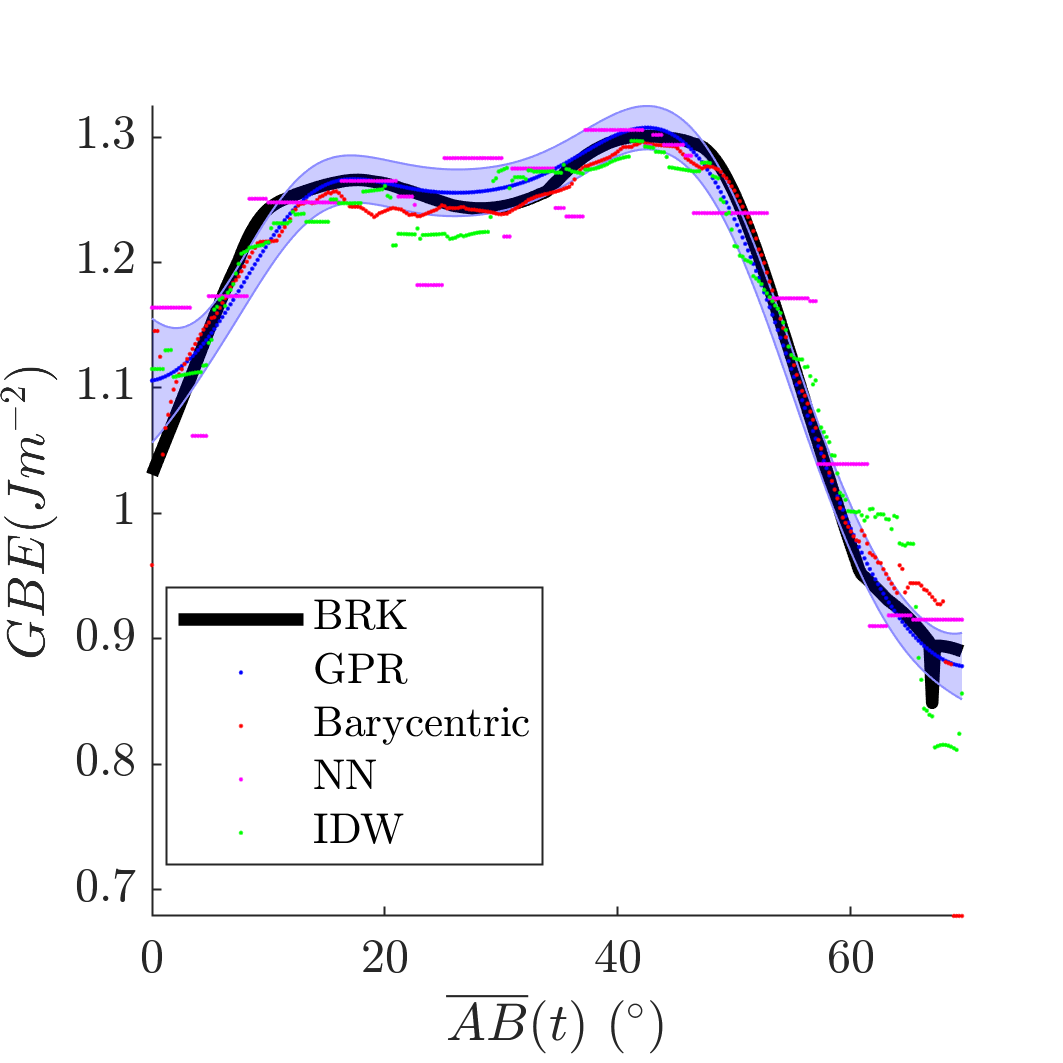
\includegraphics{figures/tunnel-50000.png}
    \caption{Predictions of \gls{gpr} (blue circles), barycentric (red circles), \gls{nn} (magenta circles), and \gls{idw} (green circles) as a function of distance along a 1D arc ($\overline{AB}$) between two \glspl{vfzo} ($A$ and $B$). The true, underlying \gls{brk} function is also shown (black line). \num{50000} random \inpt{} \glspl{vfzo} were generated and used for each of the models. \num{150} equally spaced points between $A$ and $B$ were used as \outpt{} points. \gls{gpr} uncertainty standard deviation is plotted as shaded error band.}
    \label{fig:tunnel-50000}
\end{figure}

\subsection{Interpolation Efficiency}
\label{sec:results:efficiency}

% general overview statement about the interpolation time and memory requirements

\Gls{gpr} is fast and has lower error compared to barycentric interpolation; however, the entire process has to be reevaluated (in current implementation) if the input points (i.e. \glspl{vfzo}) or input property values (i.e. \glspl{gbe}) change
(typically referred to as predictors and responses, respectively, in the machine learning community).
On the other hand, barycentric interpolation is fast if the triangulation and intersections are pre-computed and only input property values change (see \texttt{interp\_bary\_fast.m}), but slow if the \inpt{} or \outpt{} points change, which requires recomputing the triangulation and intersections.

Computational runtimes of the various interpolation methods are also shown (\cref{tab:runtime}). Barycentric interpolation takes the longest, in spite of the fact that it is the only parallelized method by default (not accounted for in \cref{tab:runtime}). In other words, since 12 cores were used to obtain these runtime results, the total runtime across all cores is much higher compared with the other methods; however, it is possible that other methods used multi-threading via built-in vectorized functions. The long computation times of barycentric interpolation result primarily from the large number of facets present in a high-dimensional mesh triangulation and the interconnectedness of facets with respect to each other.

\Gls{gpr} is the second-longest in terms of of runtime, but is more accurate than any of the other three methods. \Gls{nn} and \gls{idw} interpolation have vectorized implementations and are much simpler than the barycentric and \gls{gpr} methods. Consistent with expectations, \gls{nn} and \gls{idw} exhibit almost negligible runtimes; however, this is at the expense of increased error, as discussed earlier (\cref{sec:results:accuracy}). It should also be noted that barycentric interpolation has much higher memory requirements than \gls{gpr}, \gls{nn}, and \gls{idw} due to the need to store large matrices. If \texttt{fitrgp PredictMethod = 'exact'}, then \gls{gpr} also has high memory requirements for large \gls{vfzo} sets. For \num{50000} input points with sufficient RAM (e.g. 128 GB) and 12 cores available, the \texttt{'exact'} method runtime is \SI{535.1 \pm 392.6}{seconds}.

Because the default implementation of \gls{idw} uses a radius cut-off, the distance and weight matrices can be stored as sparse objects, dramatically reducing both the storage requirements and computational complexity of this method. We expect that a \gls{knn} approach would produce similar results both in terms of runtime and error when a relatively uniform sampling of \gls{gbc} is obtained.

\begin{table*}
\centering
\caption{Comparison of average~runtime~(\SI{}{\second}) for \num{10} trials for barycentric, \gls{gpr}, \gls{idw}, and \gls{nn} interpolation methods for various \gls{vfzo} set sizes using 12 cores. Because \gls{gpr}, \gls{idw}, and \gls{nn} method defaults do not use \texttt{parfor} loops but may have internal multi-core vectorization, it is unclear to what extent the number of cores affects the runtime of methods other than barycentric interpolation. \Gls{vfzo} symmetrization runtime was not included; however, symmetrization of \num{50000} \glspl{gbo} takes approximately \SI{\symtime}{seconds} on \SI{6}{cores} (Intel i7-10750H, 2.6 GHz) and is a common step in every interpolation method (i.e. it is fundamental to the \gls{vfzo} framework).}
\label{tab:runtime}
\begin{tabular}{lllll}
\cline{2-5}
                    & \multicolumn{4}{c}{Runtime (s)}                                                     \\ \hline
\gls{vfzo} Set Size & Barycentric       & GPR                 & IDW                 & NN                  \\ \hline
\num{100}           & $191.8 \pm 19.57$ & $0.4187 \pm 0.4342$ & $0.034 \pm 0$       & $0.0367 \pm 0.0041$ \\
\num{388}           & $388.4 \pm 18.84$ & $0.943 \pm 0.3481$  & $0.0904 \pm 0.0224$ & $0.0705 \pm 0.0129$ \\
\num{500}           & $455.7 \pm 55.28$ & $0.6104 \pm 0.3138$ & $0.1352 \pm 0.0364$ & $0.0724 \pm 0.0051$ \\
\num{1000}          & $536.5 \pm 35.26$ & $1.743 \pm 0.9464$  & $0.1948 \pm 0.0395$ & $0.1203 \pm 0.0184$ \\
\num{5000}          & $998.9 \pm 54.48$ & $5.216 \pm 0.4816$  & $0.8726 \pm 0.1529$ & $0.9277 \pm 0.2418$ \\
\num{10000}         & $1516 \pm 56.59$  & $5.609 \pm 0.8756$  & $1.631 \pm 0.3915$  & $0.8938 \pm 0.1717$ \\
\num{20000}         & $2526 \pm 119.5$  & $11.45 \pm 3.29$    & $3.191 \pm 0.4752$  & $1.275 \pm 0.3423$  \\
\num{50000}         & $5743 \pm 361.3$  & $13.69 \pm 4.05$    & $7.635 \pm 1.872$   & $3.817 \pm 0.5884$  \\ \hline
\end{tabular}
\end{table*}

\subsection{Simulation Dataset}
\label{sec:results:simulation}
Interpolation results for a large database of Fe \gls{gbe} simulations \cite{kimPhasefieldModeling3D2014} are presented in \cref{fig:kim-interp}, where approximate coordinates for the octonions $A$ and $B$ in \cref{fig:kim-interp}b are given in \cref{tab:tunnel-AB2}). A \gls{gpr} mixture model (\cref{fig:kim-interp-teach}) based on a sigmoid mixing function (\cref{fig:gprmix-sigmoid}) that builds on the \gls{gpr} interpolation scheme discussed in this work is used to better predict low \gls{gbe} values of the noisy dataset. If multiple metastable \glspl{gbe} (e.g. 3-10 metastable states per distinct \gls{gb} rather than a single metastable \gls{gbe}) were available and/or the \glspl{gb} were sampled more uniformly in \gls{5dof} space, the \gls{gpr} mixing scheme may not have been needed to improve predictive performance of low \glspl{gbe}. For example, \gls{gpr} in \cref{fig:brkparity50000}a shows reasonable predictive performance of low \glspl{gbe}, but the \glspl{gb} are more uniformly sampled and the \inpt{} and \outpt{} data are noise-free (compare with the poor predictions for low \gls{gbe} for this data set shown in \cref{fig:kim-interp-teach}d).

First, the Fe simulation data is obtained from \cite{kimPhasefieldModeling3D2014} rather than \cite{kimIdentificationSchemeGrain2011} due to a mistake in the earlier dataset file\footnote{We were informed of the error during an email discussion with the corresponding author of \cite{kimPhasefieldModeling3D2014}.}. First, \glspl{gb} with a \gls{gbe} less than \SI{0.01}{\joule\per\square\meter} are removed to get rid of "no-boundary" \glspl{gb}. Repeated \glspl{gb} are then identified and removed by converting all \glspl{gb} into a \gls{vfzo} set (see \texttt{Kim2oct.m}) and applying \texttt{avgrepeats.m} with \texttt{avgfn='min'} to sort the repeated \glspl{gb} into "degenerate sets"\footnote{A degenerate "set" is distinct from a \glspl{vfzo} "set", the former of which is discussed in greater detail in Supplementary Information \cref{sec:supp:kim-interp:quality}. }, and only the average \gls{gbe} (and a single \gls{gb}) within each degenerate set was retained. We estimate the intrinsic \gls{rmse} and \gls{mae} of the Fe simulation dataset to be \SIlist{0.06529;0.06190}{\joule\per\square\meter}, respectively. Minimum and maximum error was \SIlist{-0.2625;0.2625}{\joule\per\square\meter}, respectively. See \cref{sec:supp:kim-interp:quality} for further details on methods used to estimate intrinsic error of the Fe simulation dataset.

An exponential rather than a squared exponential kernel was used for the subset \gls{gpr} model (\cref{sec:supp:kim-interp}) to accommodate sharper transitions to better approximate low \glspl{gbe}. Further details of the \gls{gpr} mixture model are given in Supplementary Information (\cref{sec:supp:kim-interp}). Because only a single metastable state was used for each \gls{gbe} simulation, both the training and validation data are subject to noise, consistent with a wide lateral spread of predictions in both \cref{fig:kim-interp} and the intrinsic error estimation (\cref{fig:kim-interp-degeneracy-results}). The Fe simulation dataset \gls{gpr} mixture model gives lower \gls{rmse} (\SI{0.055035}{\joule\per\square\meter}) and \gls{mae} (\SI{0.039185}{\joule\per\square\meter}) than the intrinsic error estimates. This indicates that the intrinsic error itself is somewhat overestimated\footnote{The \outpt{} error of a model typically cannot be less than the noise of the \outpt{} data of a model even if the model is estimating the true \outpt{} values with better accuracy than the noise (which is very possible and even expected with \gls{gpr} models and Guassian noise in the \inpt{} data).}. The fact that both model and intrinsic error metrics are relatively close and that the parity plots (\cref{fig:kim-interp} and \cref{fig:kim-interp-degeneracy-results}b) also suggests that the model is performing well and that further improvements in the model relative to the "true" values will be "hidden", i.e. they will probably not manifest as lower \gls{rmse} or \gls{mae} nor as more tightly distributed parity plots, etc.

% In numerical tests and consistent with our expectation, we determine that \gls{gpr} approximates the \gls{brk} validation function better than other methods when Gaussian noise is added to the training data and that parity plots have similar features to \cref{fig:kim-interp} when noise is also present in the true values. 

Given the theoretical existence of a true minimum \gls{gbe}, the predictions can be assumed to have an overprediction bias relative to the true minimum. On average, we expect this overprediction bias relative to the true minimum \gls{gbe} (rather than the most likely metastable state) may be on the order of a few hundred \SI{}{\milli\J\per\square\meter} and may vary as a function of true minimum \gls{gbe}. In other words, the model provided is probably an estimate of the most likely metastable \gls{gbe} rather than the true minimum \gls{gbe}. This is akin to saying we're providing a model that approximates the non-equilibrium, Stillinger quenched red curve of Figure 4(c1) in \cite{hanGrainboundaryMetastabilityIts2016}, not the minimum \gls{gbe} blue curve of the same chart. See \cite{hanGrainboundaryMetastabilityIts2016} for an in-depth treatment of equilibrium and metastable \gls{gbe}.

Again, data for which multiple metastable \glspl{gbe} (e.g. 3-10 repeats) are provided for each \gls{gb} will likely greatly improve the performance of the \gls{gpr} model in predicting either most likely metastable \gls{gbe} (when all \glspl{gbe} are considered) or true minimum \gls{gbe} (when only the minimum \gls{gbe} is considered for each \gls{gb}) and may even negate the need for a \gls{gpr} mixture approach. Thus, where feasible, we hope that future large-scale \gls{gb} bicrystal simulation studies will report all property data for repeated trial runs rather than a single trial run or a single value from a set of trial runs. Ideally, data for the three additional microscopic \glspl{dof} for \glspl{gb} (which falls into the category of epistemic uncertainty in this work) would also be included. We believe it is likely that minimum energy paths (i.e. paths of steepest descent) in the \gls{gbe} landscape depend on both macroscopic and microscopic \glspl{dof} (in total, 8DOF) and could offer a more holistic view of \gls{gb} behavior that better mimics and explains experimental grain growth observations.

The model can be probed at new \glspl{gb} via \texttt{gprmix.m}, which provides both predicted \gls{gbe} and uncertainty standard deviation. A subject of future study in our group is to use this model for grain growth simulations.

\begin{figure*}
    \centering
    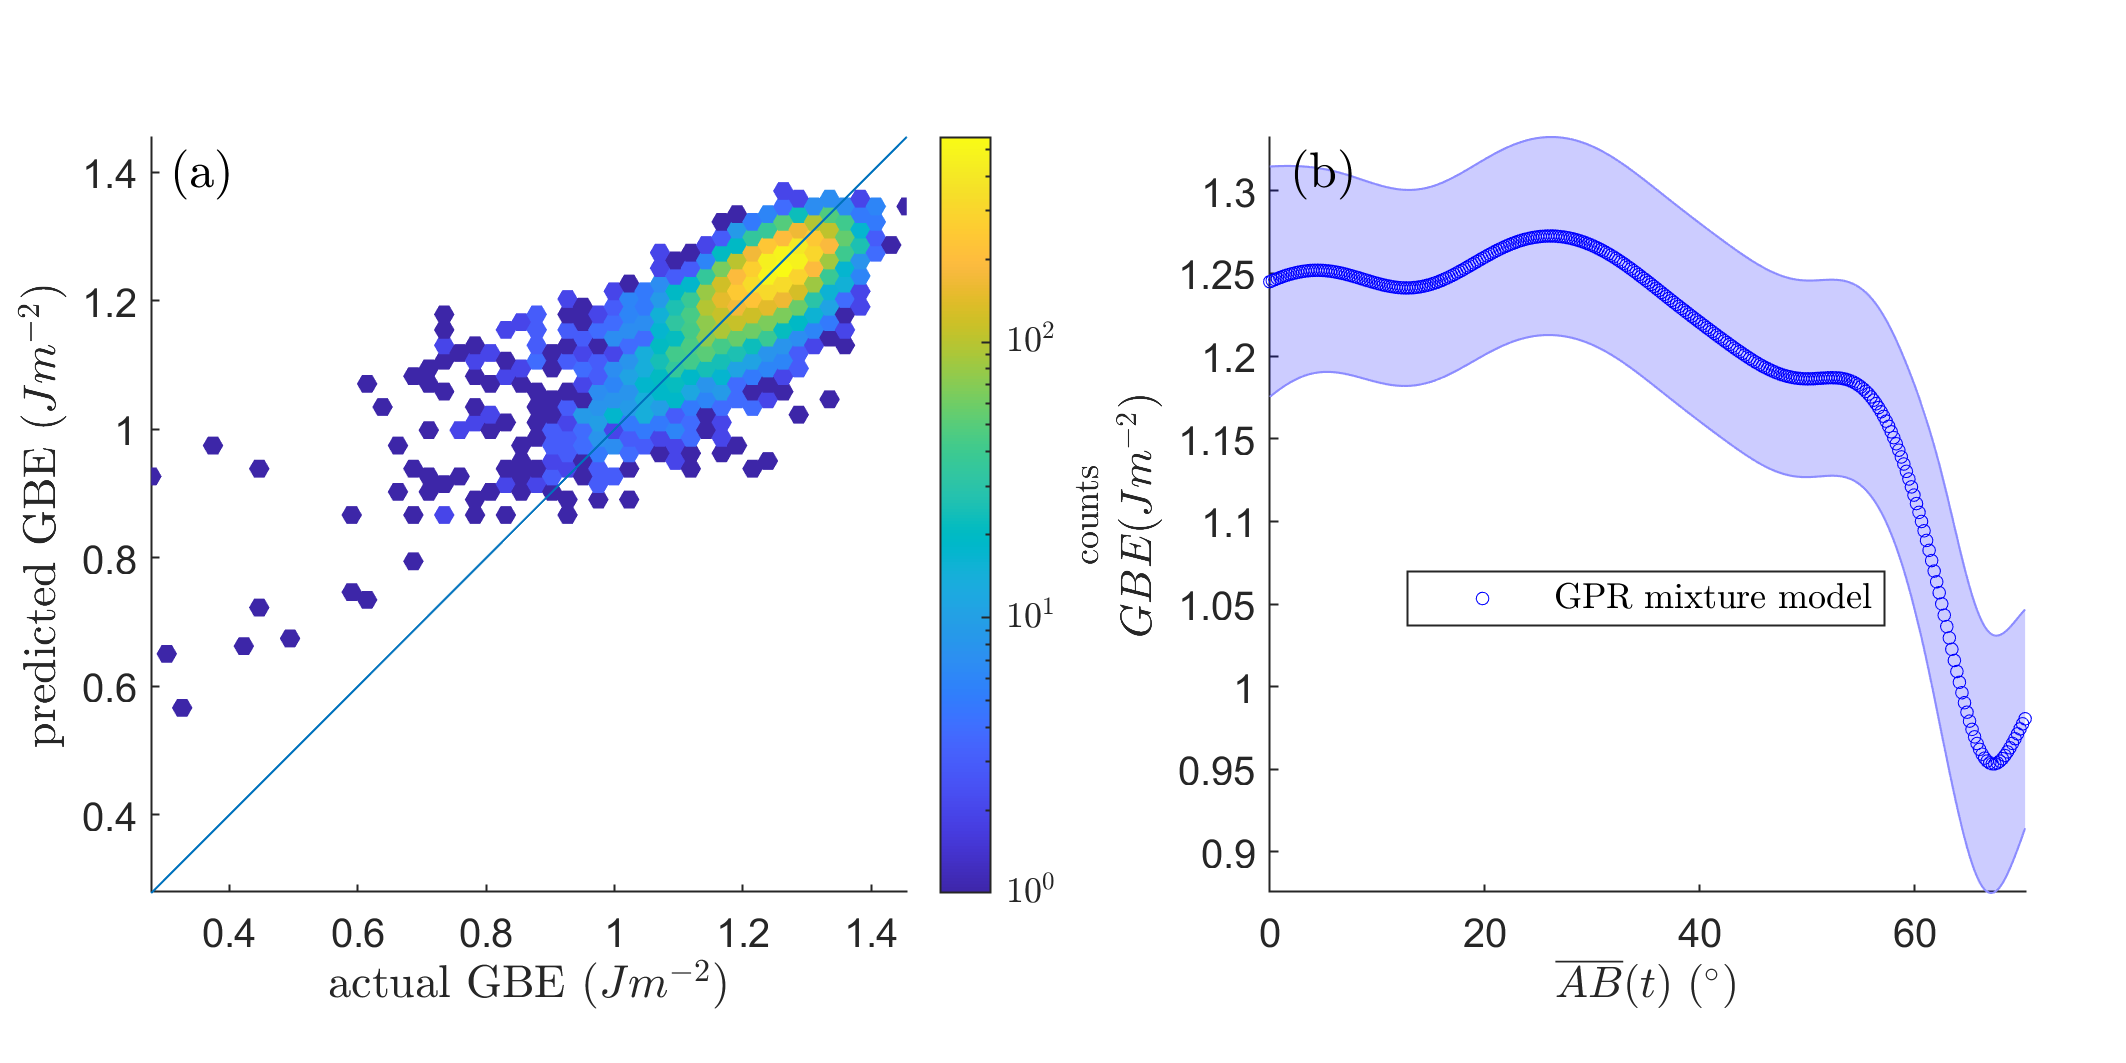
\includegraphics{kim-interp.png}
    \caption{Interpolation results for a large Fe simulation database \cite{kimPhasefieldModeling3D2014} using \num{46883} \inpt{} \glspl{gb} and \num{11721} \outpt{} \glspl{gb} in an 80\%/20\% split and a \gls{gpr} mixture model to better approximate low \glspl{gbe}. Use of a \gls{gpr} mixture model predicts low \gls{gbe} better than the standard \gls{gpr} model (compare with \cref{fig:kim-interp-teach}d). Hexagonally binned parity plot of the \gls{gpr} mixing model with \gls{rmse} and \gls{mae} of \SIlist{0.055035;0.039185}{\J\per\square\meter}, respectively, relative to typical, constant average models of \SIlist{0.0854;0.0617}{\joule\per\square\meter}, respectively (a). Predictions of \gls{gpr} mixture model (blue circles) as a function of distance along a 1D arc ($\overline{AB}$) between two \glspl{vfzo} ($A$ and $B$) (b). }
    \label{fig:kim-interp}
\end{figure*}

\begin{table*}
\centering
\caption{Approximate coordinates of \glspl{vfzo} $A$ and $B$ used for the Fe simulation interpolation in \cref{fig:kim-interp}. Individual quaternions of each octonion are given in the laboratory reference frame with an assumed \gls{gb} normal pointing in the +z direction, also in the laboratory reference frame.}
\label{tab:tunnel-AB2}
\begin{tabular}{lllllllll}
\hline
Octonion & o(1)   & o(2)    & o(3)    & o(4)    & o(5)    & o(6)   & o(7)    & o(8)   \\ \hline
A        & 0.8716 & -0.4124 & -0.1857 & 0.1893  & 0.3146  & 0.8359 & -0.3815 & 0.2382 \\
B        & 0.4391 & -0.7856 & -0.4142 & -0.1360 & -0.1376 & 0.8082 & -0.3705 & 0.4366 \\ \hline
\end{tabular}
\end{table*}

\section{Conclusion} \label{sec:conclusion}

In this work, we presented the \gls{vfzo} framework for computing distances between GBs and predicting the properties of GBs from existing measurements. We found that distance calculations in the \gls{vfzo} framework (via \vfzorepo{} function \texttt{\distfn{}.m}) are dramatically more computationally efficient ($O(N_p^2L)$) than traditional methods ($O(N_p^4L^2)$) at the expense of infrequent, large distance overestimation which can be addressed through ensemble techniques at a small computational cost (relative to traditional methods) as discussed in \cref{sec:methods:vfz-dist}.

We also developed and tested a barycentric interpolation method, and adapted three other interpolation methods for use in the \gls{vfzo} framework. We provide an easy-to-use, versatile implementation of our methods through an interpolation function \texttt{interp5DOF.m} written in MATLAB  (\url{github.com/sgbaird-5dof/interp}, \cite{bairdFiveDegreeofFreedom5DOF2020}) and many companion functions in the \vfzorepo{}.  This approach is general and applies to any crystal system (any of the 32 crystallographic point groups can be selected by the parameter \texttt{pgnum}). 

Of the interpolation methods that we present in this work, \Gls{gpr} provided the highest accuracy predictions. It also provided higher accuracy predictions than any of the methods in the literature. The \gls{gpr} interpolation errors (\num{50000} \glspl{vfzo}) for the \gls{brk} validation model are about 2.4 times the intrinsic error that would be expected from noise-free reconstruction of polycrystalline data via \gls{lobpcg} \cite{shenDeterminingGrainBoundary2019} (\num{180000} \glspl{gb}) with their (simpler) validation model. Moreover, the interpolation errors for a Fe simulation dataset are on par with the intrinsic errors of the dataset itself (\cref{sec:supp:kim-interp:quality}). While \gls{idw}, and \gls{nn} interpolation, have the fastest computation times, they also have higher interpolation error. Consequently, we recommend the \gls{gpr} interpolation method for the \gls{vfzo} framework for most applications because it provides the best combination of accuracy and speed and handles \inpt{} noise; however, the other methods can meet niche needs. For example, barycentric interpolation enables rapid and accurate predictions when the function to be evaluated changes, but the \inpt{} and \outpt{} \glspl{gb} remain fixed. 

We anticipate that the \gls{vfzo} framework and corresponding implementation will benefit numerous applications related to \gls{gb} structure and properties, including facilitating \gls{gb} structure-property model development, enabling efficient surrogate modeling of \gls{gb} properties, and larger scale iterative simulations that require repetitive evaluation of computationally expensive structure-property models.

\section*{Acknowledgement}
\label{sec:acknowledgement}

The authors thank Ian Chesser, Toby Francis, Victoria Baird, and Brandon Snow for useful discussions. The material presented here is based upon work supported by the National Science Foundation under Grant No. 1610077.

% \appendix
\label{sec:app}
\section{Detailed Barycentric Interpolation Methods}
\setcounter{figure}{0}
\subsection{Triangulating a \glsentrytitlecase{vfz}{long} Mesh}
\label{app:bary-tri}

% Briefly (but clearly and explicitly) explain the steps of generating the cubochorically sampled GBs, converting them to octonions and then mapping all of them into the vfz. Then explain how you do the triangulation. This will require a few figures to show the process in 3D (i.e. generating a triangulation of a point cloud on a region of the surface of the 2-sphere).

% After random \glspl{vfzo} are obtained (\cref{sec:methods:rand}), % ...

In order to reduce the computational complexity of triangulating a high-dimensional mesh \cite{barberQuickhullAlgorithmConvex1996}, some simplifications are made. The degenerate dimension obtained from analytically minimizing $U(1)$ symmetry \cite{francisGeodesicOctonionMetric2019} is first removed via a rigid (i.e. distance- and angle-preserving) \gls{svd} transformation,
%to enable use of MATLAB's quickhull \cite{barberQuickhullAlgorithmConvex1996} implementations such as \texttt{delaunayn} and \texttt{convhulln}. Removal of the degenerate dimension is done via a rigid \gls{svd} transformation,
analogous to a Cartesian rotation and translation
%Thus, a set of octonions originally represented by 8D Cartesian coordinates are collapsed to a 7D Cartesian representation while preserving both distances and angles among the points
As a 3D Cartesian to 2D Cartesian analogue of this 8D Cartesian to 7D Cartesian transformation, we take a set . Next, this 7D Cartesian representation is projected onto a hyperplane tangent to the mean of the input points\footnote{This is \textit{not} a rigid transformation; however, it is sufficiently close to produce a high-quality triangulation in a \gls{vfz}.} (\cref{fig:bary-delaunay}b). The 7D Cartesian \glspl{gbo} undergo another rigid \gls{svd} transformation to 6D Cartesian (see 3D to 2D analogue in \cref{fig:bary-delaunay}c) for which a triangulation is computed via the quickhull algorithm \cite{barberQuickhullAlgorithmConvex1996} (see MATLAB function \texttt{delaunayn}).

\begin{figure}
    \centering
    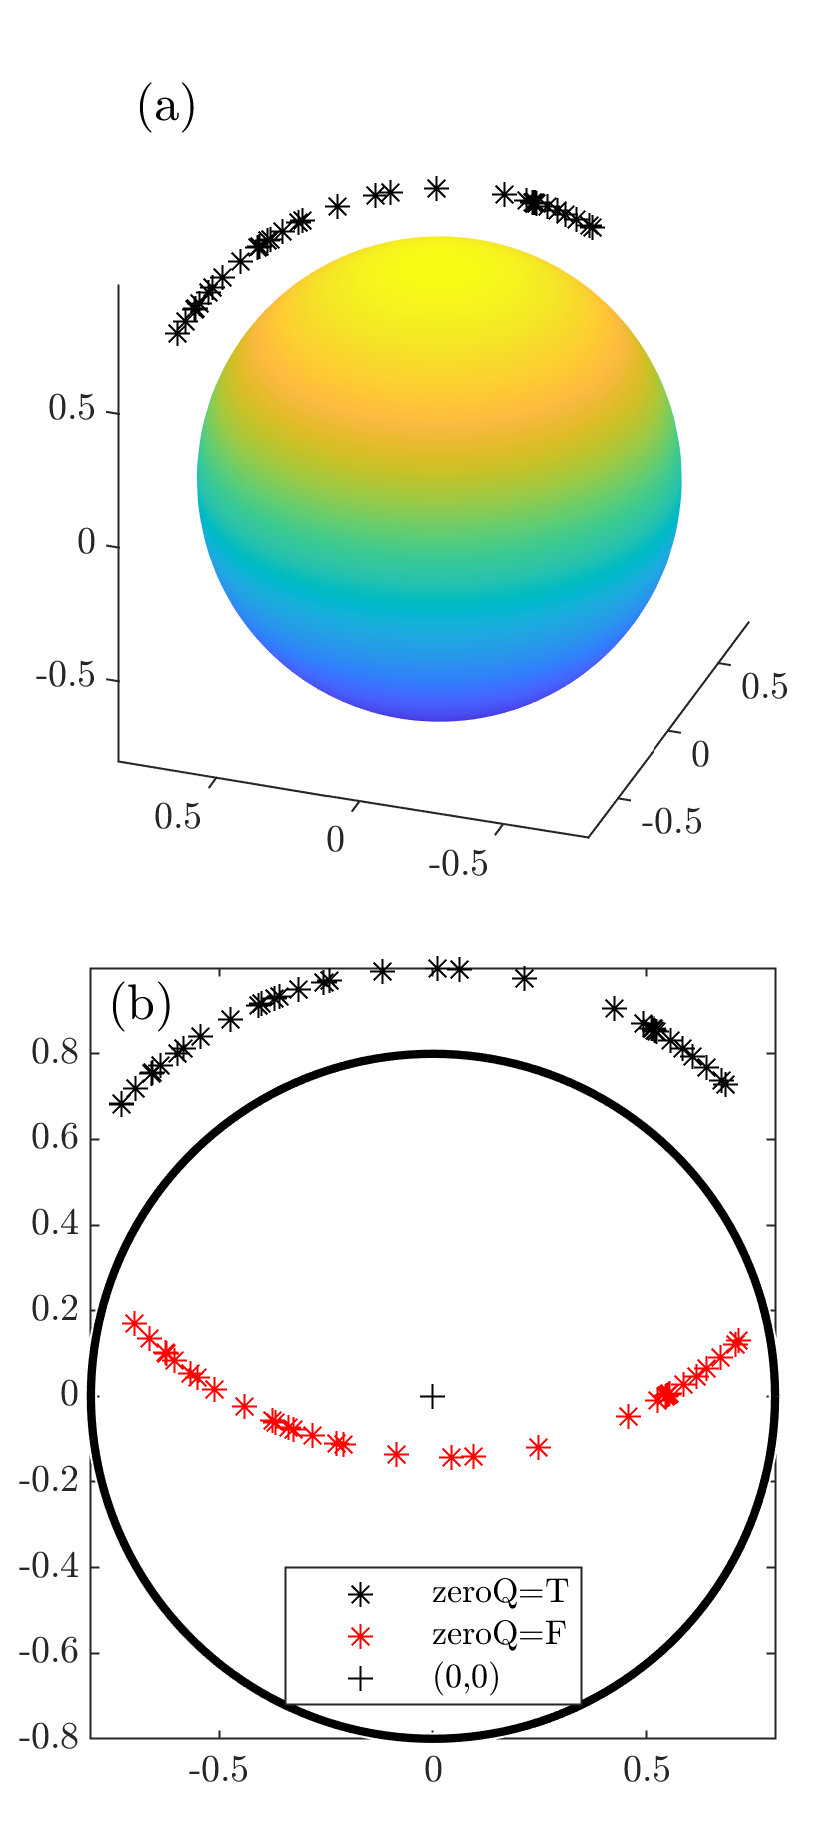
\includegraphics[scale=1]{bary-remove-deg.png}
    \caption{3D Cartesian to 2D Cartesian analogue of 8D Cartesian to 7D Cartesian degeneracy removal used in barycentric interpolation approach. Starting spherical arc points on surface of 2-sphere (a) and degenerate dimension removed via \acrlong{svd} transformation to 2D Cartesian (b) with either the origin (black plus) preserved (black asterisks, \texttt{zeroQ=T}) or ignored (red asterisks, \texttt{zeroQ=F}). The sphere (a) and circle (b) each have a radius of 0.8 and are used as a visualization aid only.}
    \label{fig:bary-remove-deg}
\end{figure}

Using a separate rigid \gls{svd} transformation from the triangulation, the original mesh and prediction \glspl{gbo} are simultaneously transformed from 8D Cartesian to 7D Cartesian. Because our \gls{svd} approach is rigid, the triangulation is then superimposed onto the newly transformed input points resulting in a 7D Cartesian \gls{vfz}.

\begin{figure}
    \centering
    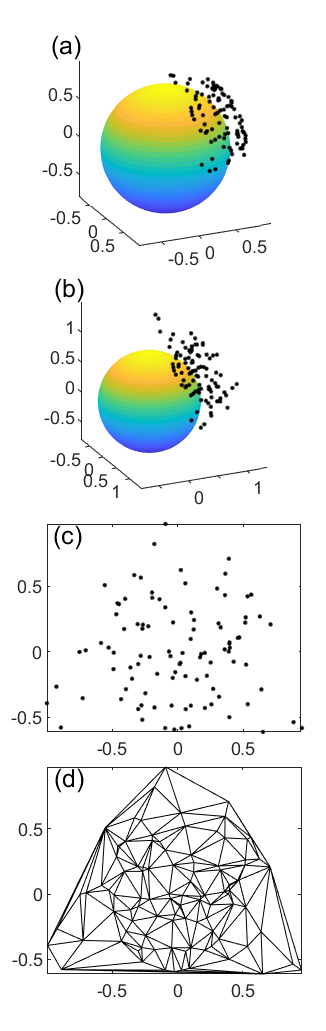
\includegraphics[scale=1]{bary-delaunay.png}
    \caption{3D Cartesian to 2D Cartesian analogue of 7D Cartesian to 6D Cartesian mesh triangulation used in barycentric interpolation approach. Input points linearly projected projected onto hyperplane tangent to mean of starting points (a), degenerate dimension removed via rigid \gls{svd} transformation to 2D Cartesian and Delaunay triangulation calculated (b), and Delaunay triangulation superimposed onto normalized input points. The spheres in (a) and (c) have a radius of 0.8 and is used for visualization only.}
    \label{fig:bary-delaunay}
\end{figure}

% In order to reduce the computationally complexity of computing barycentric coordinates in a high-dimensional space \cite{barberQuickhullAlgorithmConvex1996}, a single degenerate dimension (originally introduced by analytically minimizing $U(1)$ symmetry) is removed to enable use of MATLAB's quickhull \cite{barberQuickhullAlgorithmConvex1996} implementations such as \texttt{delaunayn} and \texttt{convhulln}. Removal of the degenerate dimension is done via a rigid \gls{svd} transformation, analogous to a Cartesian rotation and translation. Thus, a set of octonions originally represented by 8D Cartesian coordinates are collapsed to a 7D Cartesian representation while preserving both distances and angles among the points (see 3D to 2D analogue in \cref{fig:bary-remove-deg}). To further reduce the "curse of dimensionality" in computing the triangulation, a 7D Cartesian representation of the octonions constrained to lie on the surface of the 6-sphere are first projected onto a hyperplane tangent to the mean of the input points and then rotated/translated again via \gls{svd} to produce a 6D Cartesian representation (see 3D to 2D analogue in Figure \cref{fig:bary-delaunay}). This 6D representation is used to compute a triangulation via the built-in MATLAB routine \texttt{delaunayn} based on the quickhull algorithm \cite{barberQuickhullAlgorithmConvex1996}, giving facet vertices for the 7D Cartesian hypersphere.

\subsection{Intersections in a \glsentrytitlecase{vfz}{long} Mesh}
\label{app:bary-int}
An intersection is calculated by linearly projecting a prediction point onto the hyperplane defined by a mesh facet's vertices (\cref{fig:bary-interp}, computing barycentric coordinates within the facet, and testing for positivity \cite{langerSphericalBarycentricCoordinates2006}, and repeating this process until an intersection is found or a stop condition is reached (see \texttt{nnMax} below). If the prediction point is contained within the simplex, all of the barycentric weights (i.e. coordinates) are positive. If it outside the simplex, this constraint is violated. Due to the large number of facets per point of a high-dimensional
%simplex-based
triangulation
%and for computational speed,
prediction point intersections are calculated by considering facets connected to up to some number of mesh \glspl{nn} (\texttt{nnMax}) (in this work, \texttt{nnMax = 10}). For prediction points where no intersecting facet is found
%in these connected facets due to high-aspect ratio facets or prediction point falling outside the mesh within a given tolerance,
a \gls{nn} approach is used (\cref{sec:methods:interp:nn}), which represent average non-intersection rates of \SI{0.1207 \pm 1.02}{\percent} and \SI{0.68 \pm 0.11}{\percent} for input meshes of \num{388} and \num{50000}, respectively, for \num{10000} query points out of \num{10} trials.

\subsection{Interpolation via Barycentric Coordinates}
\label{app:bary-interp}

Once barycentric coordinates are computed for a prediction point within the input mesh, the interpolated value is found by taking the dot product of the barycentric coordinates and the properties of the corresponding vertices of the intersecting facet via
\begin{equation}
\label{eq:bary-interp}
v=\underset{i=1}{\overset{N}{\sum }}\lambda _i v_i
\end{equation}
where $\lambda$, $v$, $v_i$ and $N$, are the barycentric coordinates, interpolated property, property of the $i$th vertex of the intersecting facet, and number of vertices in a given facet ($N = 7$ for the degeneracy-free 6-sphere). A 2-sphere example is provided in \cref{fig:bary-interp}.

\begin{figure}
    \centering
    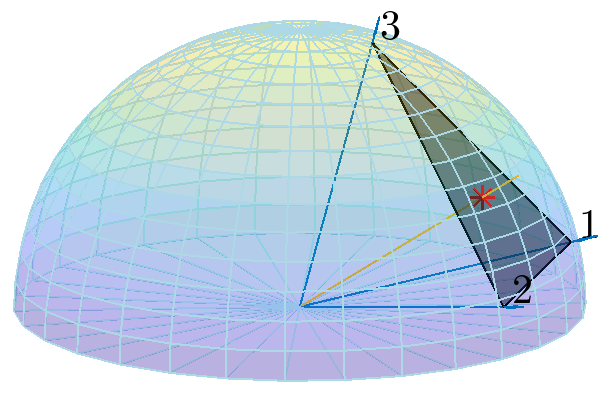
\includegraphics[scale=1]{bary-interp.png}
    \caption{A ray (red line) on the 2-sphere is linearly projected onto the hyperplane of a mesh facet (transparent black), shown as a red asterisk. The barycentric coordinates are computed as $\lambda_{i \in [1,3]} = \frac{1}{3}$. Because all barycentric coordinates are positive, it is determined that the projected point is an intersection with the mesh. Given vertex values of \num{8.183}, \num{3.446}, and \num{3.188} for vertices 1, 2, and 3, respectively, the interpolated value is calculated as \num{4.94} via \cref{eq:bary-interp}.}
    \label{fig:bary-interp}
\end{figure}

% \appendix
\begin{appendices}

\crefalias{section}{appsec}
\crefalias{subsection}{appsec}
\crefalias{subsubsection}{appsec}

\section{Detailed Barycentric Interpolation Method}
\label{sec:app}
\renewcommand\thefigure{\thesection.\arabic{figure}} 
\setcounter{figure}{0}

We describe barycentric interpolation applied in the \gls{vfzo} framework in more detail. This includes:
\begin{itemize}
    \item[1] triangulation of a \gls{vfz} mesh (\cref{sec:app:bary:tri})
    \item[2] finding intersections between arbitrary \glspl{vfzo} and the \gls{vfz} mesh (i.e. finding intersecting facets) (\cref{sec:app:bary:int})
    \item[3] calculating interpolated values of an arbitrary \gls{vfzo} property using the intersecting facet (\cref{sec:app:bary-interp})
\end{itemize}

\subsection{Triangulating a \glsentrytitlecase{vfz}{long} Mesh}
\label{sec:app:bary:tri}

Creation of a simplicial mesh is necessary to perform barycentric interpolation. Due to the difficulty of visualizing a 7-sphere, we provide visual illustrations of the process as applied to lower-dimensional analogues. After \glspl{gbo} have been symmetrized into a \gls{vfz} (\cref{sec:methods:framework:vfz}), the triangulation process is as follows:
\begin{enumerate}
    \item[1.1] Apply a \gls{svd} transformation to remove the U(1)-symmetry degeneracy inherent in the \gls{vfzo} coordinates (\cref{sec:app:bary:tri:svd1})
    \item[1.2] To reduce computational burden of the triangulation, linearly project \glspl{vfzo} onto a hyperplane that is tangent to the vector between the origin and the mean of the \inpt{} \glspl{vfzo}
    \item[1.3] Perform a second \gls{svd} transformation (\cref{sec:app:bary:tri:svd2})
    \item[1.4] Compute the triangulation according to the quickhull algorithm \cite{barberQuickhullAlgorithmConvex1996} using built-in methods
\end{enumerate}

In the explanation of each of these steps that follows, e make reference to lower-dimensional visual analogues of the \gls{vfzo} triangulation procedure, which are given in \cref{fig:bary-remove-deg}, \cref{fig:bary-delaunay}, and \cref{fig:bary-interp}. We note that 3D Cartesian coordinates in \cref{fig:bary-remove-deg} correspond to 8D Cartesian coordinates, whereas 3D Cartesian coordinates in \cref{fig:bary-delaunay} and \cref{fig:bary-interp} correspond to 7D Cartesian coordinates. This is intentional for two reasons:
\begin{itemize}
    \item \cref{fig:bary-remove-deg} illustrates that unsymmetrized 8D Cartesian \glspl{gbo} are analogous to a point cloud on the 2-sphere (\cref{fig:bary-remove-deg}a) and that a 8D Cartesian \gls{vfzo} set, which has already been symmetrized, is analogous to a geodesic arc on the 2-sphere (\cref{fig:bary-remove-deg}b). A \gls{vfzo} set has a degenerate dimension that can then be removed by a rigid \gls{svd} transformation to 7D Cartesian coordinates (analogous to 2D Cartesian coordinates in \cref{fig:bary-remove-deg}c). This sequence would be more difficult to visualize if \cref{fig:bary-remove-deg}a was meant to represent a point cloud on the 3-sphere (4D Cartesian coordinates), etc.
    \item \cref{fig:bary-delaunay} illustrates a second \gls{svd} transformation from normalized 7D Cartesian coordinates (\cref{fig:bary-delaunay}a) to 6D Cartesian coordinates (\cref{fig:bary-delaunay}b). Key issues are retained that would otherwise be lost (\cref{sec:supp:bary:artifact}) if an arc on a circle (1-sphere) to 1D Cartesian coordinates were used instead\footnote{Non-intersection issues due to high-aspect ratios and consideration of facets connected up to \texttt{nnMax} \glspl{nn} do not manifest in triangulations on the surface of a 1-sphere because one of the two facets (i.e. line segments) connected to the first \gls{nn} mesh vertex relative to the \outpt{} point is guaranteed to have an intersection.}. Additionally, the use of actual triangles is a more familiar and compelling illustration of \textit{triangulation}.
\end{itemize}

\begin{figure*}
    \centering
    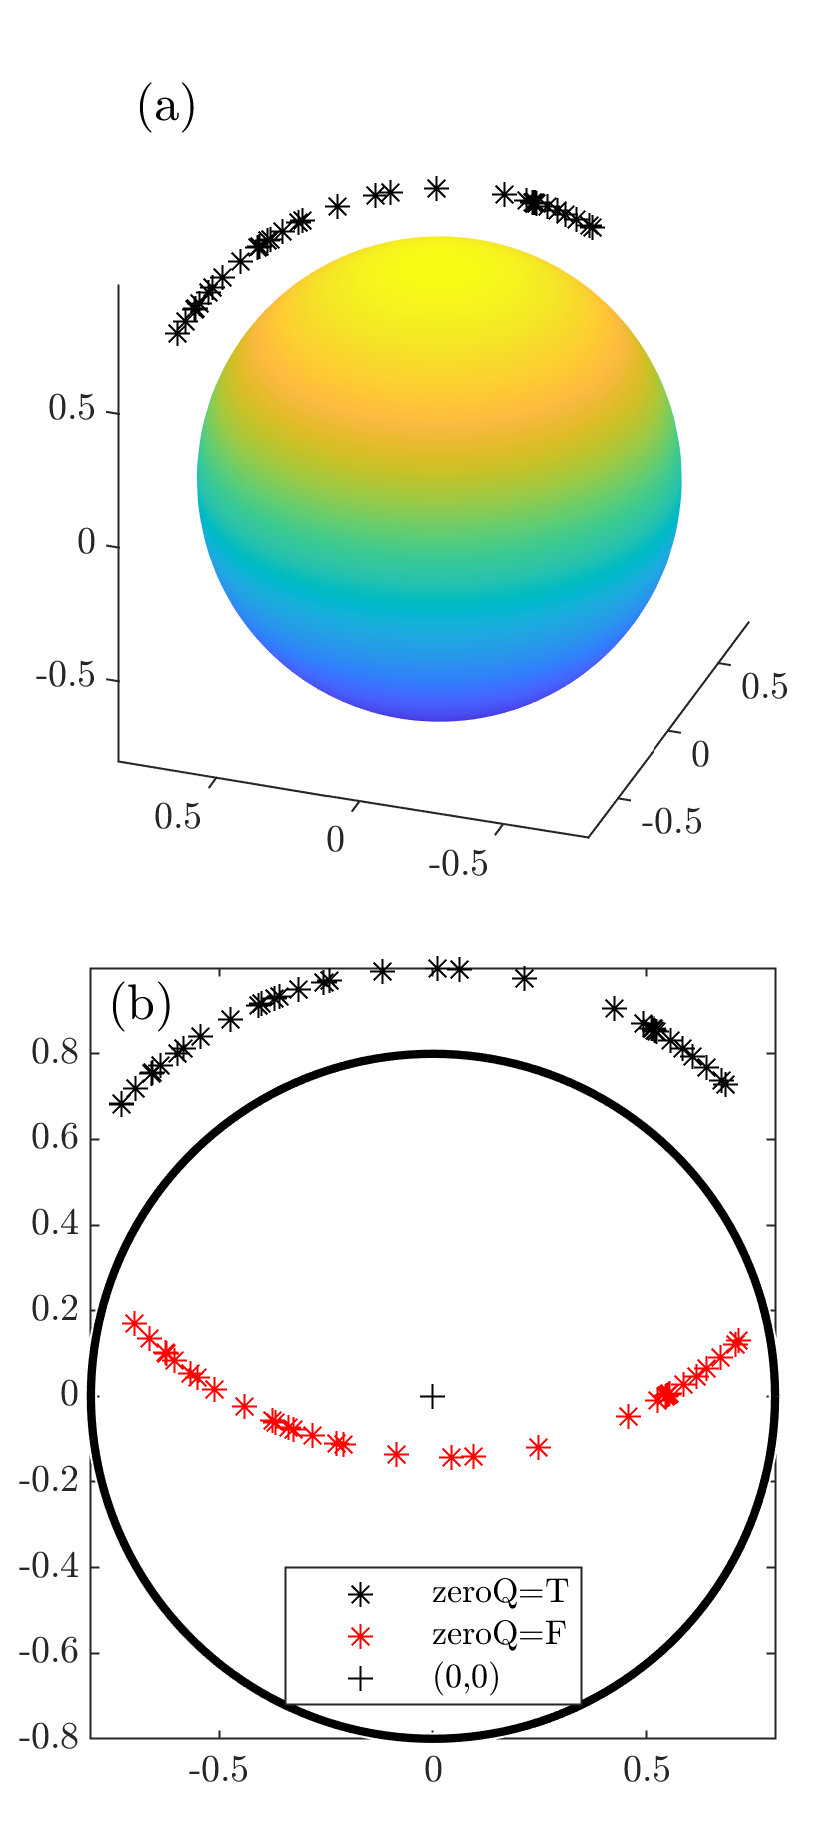
\includegraphics[scale=1]{bary-remove-deg.png}
    \caption{3D Cartesian to 2D Cartesian analogue of 8D Cartesian to 7D Cartesian degeneracy removal via rigid \gls{svd} transformation as used in barycentric interpolation approach. (a) Starting spherical arc points on surface of 2-sphere, (b) rotational symmetrization applied w.r.t. z-axis (analogous to U(1) symmetrization), and (c) degenerate dimension removed via \acrlong{svd} transformation to 2D Cartesian with either the origin (black plus) preserved (black asterisks, \texttt{zeroQ=T}) for triangulation or ignored (red asterisks, \texttt{zeroQ=F}) for mesh intersection. The spheres (a,b) and circle (c) each have a radius of 0.8 and are used as a visualization aid only.}
    \label{fig:bary-remove-deg}
\end{figure*}

\begin{figure*}
    \centering
    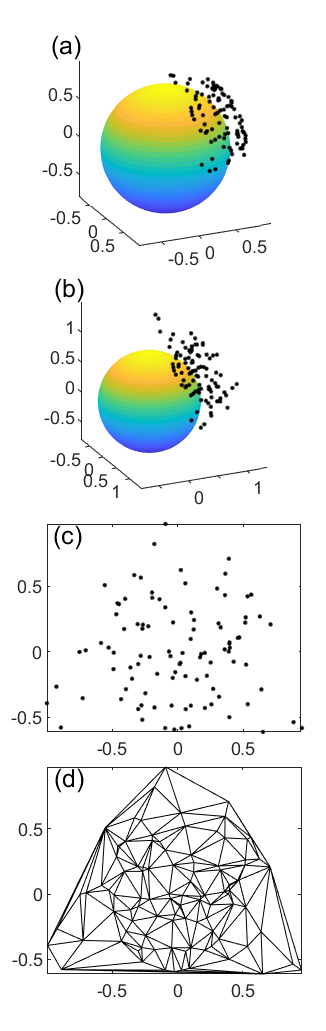
\includegraphics[scale=1]{bary-delaunay.png}
    \caption{3D Cartesian to 2D Cartesian analogue of 7D Cartesian to 6D Cartesian mesh triangulation used in barycentric interpolation approach. (a) 3D Cartesian \inpt{} points are (b) linearly projected onto hyperplane that is tangent to mean of starting points. (c) The degenerate dimension is removed via a rigid \gls{svd} transformation to 2D Cartesian and the Delaunay triangulation (black lines) is calculated, with \inpt{} vertices (red). Delaunay triangulation superimposed onto normalized \inpt{} points (d). The spheres in (a), (b), and (d) have a radius of 0.8 and are used for visualization only.}
    \label{fig:bary-delaunay}
\end{figure*}

While lower dimensional analogues are useful for visualizing and understanding the process of triangulation, a written description is also given in the following sections. As appropriate, we refer back to the teaching figures described in this section.

\subsubsection{\glsentrytitlecase{svd}{long} Transformation from 8D Cartesian to 7D Cartesian}
\label{sec:app:bary:tri:svd1}
 To reduce the computational complexity of triangulating a high-dimensional mesh \cite{barberQuickhullAlgorithmConvex1996}, some simplifications are made. First, the degenerate octonion dimension obtained from analytically minimizing $U(1)$ symmetry \cite{francisGeodesicOctonionMetric2019} is removed via a rigid (i.e. distance- and angle-preserving) \gls{svd} transformation,
%to enable use of MATLAB's quickhull \cite{barberQuickhullAlgorithmConvex1996} implementations such as \texttt{delaunayn} and \texttt{convhulln}. Removal of the degenerate dimension is done via a rigid \gls{svd} transformation,
analogous to a Cartesian rotation and translation (see 3D to 2D \gls{svd} transformation from \cref{fig:bary-remove-deg}b to \cref{fig:bary-remove-deg}c).
%Thus, a set of octonions originally represented by 8D Cartesian coordinates are collapsed to a 7D Cartesian representation while preserving both distances and angles among the points

\subsubsection{Linearly Project onto Hyperplane}
\label{sec:app:bary:tri:project}
Next, the resulting 7D Cartesian representation of each \gls{vfzo} is projected onto a hyperplane that is tangent to the centroid (i.e. mean) of the \gls{vfzo} set\footnote{This is \textit{not} a rigid transformation; however, it approximates one with sufficient accuracy to produce a high-quality triangulation in a \gls{vfz}.} (\cref{fig:bary-delaunay}a). By performing this linear projection, one of the dimensions becomes degenerate.

\subsubsection{\glsentrytitlecase{svd}{long} Transformation from 7D Cartesian to 6D Cartesian}
\label{sec:app:bary:tri:svd2}
This additional degeneracy is removed via a second \gls{svd} transformation, this time to 6D Cartesian coordinates (see 3D to 2D projection in \cref{fig:bary-delaunay}a-b). Finally, the resulting points can be triangulated via the quickhull algorithm \cite{barberQuickhullAlgorithmConvex1996} (see \vfzorepo{} function \texttt{sphconvhulln.m} and built-in MATLAB function \texttt{delaunayn()}), which relies on Euclidean distances\footnote{While the triangulation algorithm used in this work relies on Euclidean distances (the use of which is possible via the \gls{vfzo} framework), other distance metrics that are non-Euclidean \cite{morawiecDistancesGrainInterfaces2019} could potentially be incorporated into the barycentric approach such as by doing an edge-length based simplex reconstruction \cite{connorHighdimensionalSimplexesSupermetric2017,boissonnatOnlyDistancesAre2017} using the \gls{vfz} triangulation edge lengths.}. Because the simplicial mesh is defined by a list of edges between vertices for each simplicial facet, this list applies immediately to the \gls{vfzo} set in its 7D Cartesian coordinates (i.e. no reverse transformation is necessary to use the mesh on the 6-sphere in 7D).

% In order to reduce the computationally complexity of computing barycentric coordinates in a high-dimensional space \cite{barberQuickhullAlgorithmConvex1996}, a single degenerate dimension (originally introduced by analytically minimizing $U(1)$ symmetry) is removed to enable use of MATLAB's quickhull \cite{barberQuickhullAlgorithmConvex1996} implementations such as \texttt{delaunayn} and \texttt{convhulln}. Removal of the degenerate dimension is done via a rigid \gls{svd} transformation, analogous to a Cartesian rotation and translation. Thus, a set of octonions originally represented by 8D Cartesian coordinates are collapsed to a 7D Cartesian representation while preserving both distances and angles among the points (see 3D to 2D analogue in \cref{fig:bary-remove-deg}). To further reduce the "curse of dimensionality" in computing the triangulation, a 7D Cartesian representation of the octonions constrained to lie on the surface of the 6-sphere are first projected onto a hyperplane tangent to the mean of the \inpt{} points and then rotated/translated again via \gls{svd} to produce a 6D Cartesian representation (see 3D to 2D analogue in Figure \cref{fig:bary-delaunay}). This 6D representation is used to compute a triangulation via the built-in MATLAB routine \texttt{delaunayn} based on the quickhull algorithm \cite{barberQuickhullAlgorithmConvex1996}, giving facet vertices for the 7D Cartesian hypersphere.

\subsection{Intersections in a \glsentrytitlecase{vfz}{long} Mesh}
\label{sec:app:bary:int}

Once the triangulation has been determined, we need to find which facet each \outpt{} point intersects (i.e. find the intersecting facet). There are two sub-steps:
\begin{itemize}
    \item[2.1] The same rigid transformation needs to be applied to the \outpt{} points as was applied to the \inpt{} points, otherwise the \outpt{} points won't line up properly with the mesh (\cref{sec:app:bary:int:out-svd})
    \item[2.2] Facets nearby a \outpt{} point are then identified and tested for intersection (\cref{sec:app:bary:int:facets}).
\end{itemize}
\subsubsection{Apply Same \glsentrytitlecase{svd}{long} to \outpt{} Points}
\label{sec:app:bary:int:out-svd}
The positions of the \outpt{} points relative to the mesh need to be constant even after the rigid \gls{svd} transformation. %Thus, it is crucial to perform the same rigid \gls{svd} transformation (i.e. same rotation and translation) on the \outpt{} points as was applied to the \inpt{} points.
This is easily accomplished by:
\begin{itemize}
    \item[2.1a] concatenating both \inpt{} and
\outpt{} points
    \item[2.1b] using the \texttt{interp5DOF} sub-routine \texttt{proj\_down} (which depends on MATLAB's built-in \gls{svd} implementation \texttt{svd()}) to perform the transformation
    \item[2.1c] subsequently separating the transformed \inpt{} and \outpt{} points (reverse of concatenation step)
\end{itemize}

To map new points onto the mesh, the \texttt{USV} structure output by \texttt{proj\_down.m} needs to be stored and supplied in future calls to \texttt{proj\_down.m}.

% To find the barycentric coordinates or weights of a \outpt{} \gls{vfzo} relative to a \gls{vfz} simplicial mesh it is necessary to first identify which simplicial facet the point is contained in and then to compute the barycentric coordinates of the point relative to the vertices of that facet. These steps are accomplished by the following approach.

\subsubsection{Testing Nearby Facets for Intersections}
\label{sec:app:bary:int:facets}
Once the \outpt{} points are lined up properly with the mesh, the intersecting facet needs to be found. The facet containing the \outpt{} point (i.e. intersecting facet) is the one for which the point's barycentric coordinates are positive. Consequently, we determine facet affiliation by:
\begin{enumerate}
    \item[2.2a] linearly projecting the \outpt{} point onto the hyperplane defined by a mesh facet's vertices (\cref{fig:bary-interp})
    \item[2.2b] computing the point's barycentric coordinates within the facet
    \item[2.2c] testing that all coordinates are positive \cite{langerSphericalBarycentricCoordinates2006}
    \item[2.2d] repeating steps 2.2a-2.2c until an intersection is found or a stop condition is reached (see \texttt{nnMax} below).
\end{enumerate}

\begin{figure}
    \centering
    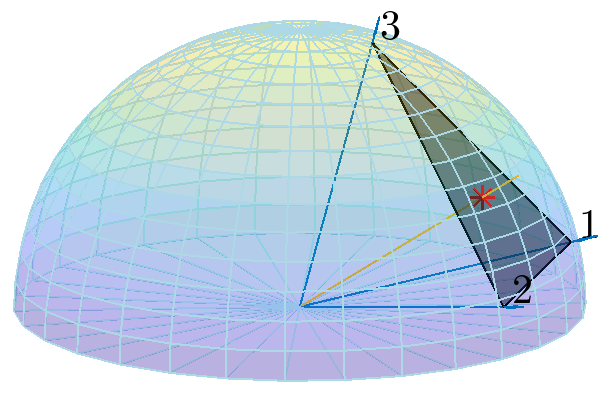
\includegraphics[scale=1]{bary-interp.png}
    \caption{A ray (red line) is linearly projected from the 2-sphere onto the hyperplane of a mesh facet (transparent black), shown as a red asterisk. The barycentric coordinates are computed as $\lambda_{i \in [1,3]} = \frac{1}{3}$. Because all barycentric coordinates are positive, it is determined that the projected point is an intersection with the mesh. Given vertex values of \num{8.183}, \num{3.446}, and \num{3.188} for vertices 1, 2, and 3, respectively, the interpolated value is calculated as \num{4.94} via \cref{eq:bary-interp}.}
    \label{fig:bary-interp}
\end{figure}

Due to the large number of facets per point of a high-dimensional triangulation (approximately \num{2000} facets per vertex for a \num{50000} point \gls{vfz} triangulation, or \num{1e8} total facets), some simplifications are made in order to determine intersections of \outpt{} points with the mesh. If every edge length of every facet were equal, only facets connected to the first \gls{nn} would need to be considered to find a proper intersection. However, since the \glspl{vfzo} are randomly sampled, edge lengths of facets are non-uniform, and non-unity aspect ratio facets exist (\cref{fig:bary-delaunay}, \cref{fig:high-aspect-non-int}). If the facets have high-aspect ratios, the intersecting facets of \outpt{} points can be far from the \glspl{nn} mesh points relative to the \outpt{} points (see \cref{fig:high-aspect-non-int} inset), especially near the perimeter of a hyperspherical surface mesh. Rather than loop through every facet to find an intersection ($~$\num{1e8} facets in \num{50000} \gls{vfzo} mesh), the \outpt{} point intersections are calculated by considering facets connected to up to some number of \gls{nn} mesh vertices (\texttt{nnMax}) relative to each \outpt{} point (in this work, \texttt{nnMax=10}). The \gls{nn} mesh vertices relative to a \outpt{} point are computed via the MATLAB built-in function \texttt{dsearchn} as in the \gls{nn} approach (\cref{sec:methods:interp:nn}). The facet IDs of facets connected to these \glspl{nn} are computed by calling built-in MATLAB function \texttt{find()} as in \texttt{find(K==nn)}, where \texttt{K} is the triangulation from \vfzorepo{} function \texttt{sphconvhulln.m} and \texttt{nn} is the ID of one of the \gls{nn} mesh vertices. 

Some \outpt{} points will have no intersecting facet found.
%(which can occur just outside the piece-wise linear perimeter of the mesh due to finite resolution)
From our numerical testing, we determined that this non-intersection phenomenon occurs in two situations:
\begin{itemize}
    \item high-aspect ratio facets (described above)
    \item \outpt{} points that are positioned just outside the bounds of the mesh but within the bounds of the \gls{vfz}, due to the fact that the mesh is a piecewise linear approximation of a surface with a curved perimeter and that randomly sampled points typically do not fall on the true perimeter
\end{itemize}
In the first case, barycentric interpolation within high-aspect ratio facets may actually lead to worse interpolation error than a \gls{nn} interpolation strategy due to influence by \glspl{gb} far from the \outpt{} point. In the second case, there is no true intersection between the \outpt{} point and the mesh. Both issues can be addressed with the same strategy: we apply a \gls{nn} approach (\cref{sec:methods:interp:nn}) when an intersecting facet is not found within \texttt{nnMax} \glspl{nn}. In numerical tests, \gls{vfz} meshes composed of \num{388} and \num{50000} vertices produced non-intersection rates of \SI{12.07 \pm 1.02}{\percent} and \SI{0.68 \pm 0.11}{\percent}, respectively, over approximately \num{10} trials and using \num{10000} \outpt{} points for each trial.

Testing intersections for nearby facets is handled in the the \vfzorepo{} function \texttt{intersect\_facet.m} and depends barycentric coordinate computations in \texttt{projray2hypersphere.m}.

\subsection{Interpolation via Barycentric Coordinates}
\label{sec:app:bary-interp}

Once a mesh triangulation has been determined (\cref{sec:app:bary:tri}) and barycentric coordinates are computed for a \outpt{} point within the \inpt{} mesh (\cref{sec:app:bary:int}), the interpolated value is found by taking the dot product of the \outpt{} point's barycentric coordinates and the properties of the corresponding vertices of the intersecting facet via
\begin{equation}
\label{eq:bary-interp}
v_{m,q}=\underset{i=1}{\overset{N}{\sum }}\lambda _{m,i} v_{m,i}
\end{equation}
where $\lambda_{m,i}$, $v_{m,q}$, $v_{m,i}$ and $N$, are the barycentric coordinates of the m-th \outpt{} point, interpolated property at the m-th \outpt{} point, property of the $i$-th vertex of the intersecting facet for the m-th \outpt{} point, and number of vertices in a given facet ($N = 7$ for facets of the simplicial mesh on the degeneracy-free 6-sphere), respectively. Interpolation of many \outpt{} points simultaneously can be accomplished by a simple, vectorized approach via MATLAB built-in function \texttt{dot()} as used in \vfzorepo{} function \texttt{interp\_bary\_fast.m}. This function assumes triangulation and weights have been precomputed. In other words, both \inpt{} and \outpt{} coordinates remain fixed, and only \inpt{} property values change. If this is the case, barycentric interpolation of new points is incredibly fast. By contrast, if \inpt{} coordinates change, the triangulation must be recomputed, and if \outpt{} coordinates change, the intersecting facets must be recomputed. Both triangulation and finding intersecting facets are computationally demanding with respect to memory and runtime (\cref{sec:results:efficiency}).
%matrix multiplication
% \begin{equation}
%     \label{eq:bary-interp_multi}
%     \mathbf{v}_q = \Lambda \mathbf{v}_m
% \end{equation}
% where $\mathbf{v}_m$ is the vector of GB properties at the mesh vertices, $\Lambda$ is the sparse matrix whose rows contain the barycentric weights for each query point, and $\mathbf{v}_q$ is the vector containing the interpolated properties at the query points.

\end{appendices}

% \newpage
\printglossaries
%need to manually clear cached files & logs in overleaf to get new abbreviations to appear

% \newpage
\bibliographystyle{elsarticle-num-names}
\bibliography{5dof-gb-energy.bib}



\end{document}
